\documentclass[a4paper,11pt,twoside]{article}
\usepackage[utf8]{inputenc}	% Text coding
\usepackage[T1]{fontenc}
\usepackage{lmodern}
\usepackage[czech]{babel}
\usepackage{epsfig}
\usepackage{amsfonts,amsmath,amssymb}
\usepackage{graphicx}
\usepackage[unicode]{hyperref}
\usepackage{indentfirst}
\usepackage{fancyhdr}
\usepackage{xifthen}
\usepackage{amsthm,thmtools}
\usepackage{bold-extra}
\usepackage[dvipsnames]{xcolor}
\usepackage[subrefformat=simple,labelformat=simple]{subcaption} % Instead of subfigure
\usepackage{listings}
\usepackage{comment}
\usepackage{titlesec}
\usepackage{underscore}
%\usepackage{showlabels}

\hypersetup{
	pdftitle={Využití počítačů ve fyzice},
	pdfauthor={Pavel Stránský},
	pdffitwindow=true,
	colorlinks=true,
	urlcolor=cyan,
	linkcolor=red,
	citecolor=green,
	filecolor=magenta
}

\graphicspath{{figures/}}

\lstdefinestyle{listingsstyle}{
    basicstyle=\ttfamily,
    breakatwhitespace=false,         
    numbersep=3,
    breaklines=true,                 
    keepspaces=true,                 
    showspaces=false,                
    showstringspaces=false,
    showtabs=false,                  
    tabsize=2,
    columns=fullflexible,
}

\lstset{style=listingsstyle}

\lstdefinestyle{TinyPython}{
    language=Python,
    basicstyle=\ttfamily\footnotesize
}

\lstdefinestyle{console}{
    basicstyle=\ttfamily\footnotesize\color{white},
    backgroundcolor=\color{black}
}

%\babelhyphenation[czech]{ma-te-ma-tic-kých}

\renewcommand\thesubfigure{(\alph{subfigure})}

\newcommand{\subsubsubsection}[1]{\paragraph{#1}\mbox{}

}

\setcounter{secnumdepth}{5}
\setcounter{tocdepth}{5}

% Page size
\addtolength{\topmargin}{-1.5cm} %\addtolength{\textheight}{-10cm}
\addtolength{\textwidth}{4cm} \addtolength{\textheight}{4cm} % Width and height of the text
\addtolength{\voffset}{-0.5cm} % Top margin
\addtolength{\hoffset}{-2cm}
\setlength{\headheight}{15pt}

\pagestyle{fancy}

\DeclareMathOperator{\e}{e}

\def\vector#1{\boldsymbol{#1}}								% Vector
\renewcommand{\d}{\mathrm{d}}
\newcommand{\derivative}[3][]{\ifthenelse{\isempty{#1}}	    % Normal derivative
	{\frac{\d{#2}}{\d{#3}}}
	{\frac{\d^{#1}{#2}}{\d{#3}^{#1}}}
}
\newcommand{\im}{\mathrm{i}}

\def\makematrix#1{\begin{pmatrix}#1\end{pmatrix}}       % Matrix
\def\abs#1{\left|#1\right|}
\def\probability#1{\mathrm{Pr}\left[#1\right]}
\def\expectation#1{\mathrm{E}\left[#1\right]}
\def\dispersion#1{\sigma_{#1}^{2}}

\def\code#1{\textnormal{\texttt{#1}}}
\def\file#1{\textnormal{\textbf{\texttt{#1}}}}
\def\ghfile#1#2{\textnormal{\textbf{\texttt{\href{https://github.com/PavelStransky/PCInPhysics2021/blob/main/#1#2}{#2}}}}}

\def\abbreviation#1{\textnormal{\textsc{#1}}}

\long\def\python#1{{\color{ForestGreen}#1}}

\newtheoremstyle{spaced}
{5pt}{5pt}{\itshape}{}{\bfseries}{:}{.5em}{}

\newtheoremstyle{red}
{5pt}{5pt}{\itshape\color{red}}{}{\bfseries\color{red}}{:}{.5em}{}

\newtheoremstyle{green}
{5pt}{5pt}{\itshape\color{ForestGreen}}{}{\bfseries\color{ForestGreen}}{:}{.5em}{}

\newtheoremstyle{blue}
{5pt}{5pt}{\itshape\color{blue}}{}{\bfseries\color{blue}}{:}{.5em}{}

\theoremstyle{red}
\declaretheorem[name=Úkol,numberwithin=section]{task}

\theoremstyle{green}
\declaretheorem[name=Úkol,numberwithin=section,sibling=task]{voluntary}

\begin{document}

\theoremstyle{spaced}
\newtheorem{example}{Příklad}[section]

\theoremstyle{blue}
\newtheorem{solution}{Řešení}[section]

\title{Zápisky k předmětu Využití počítačů ve fyzice}
\date{\today}
\author{Pavel Stránský}

\maketitle
\tableofcontents

\newcommand{\sectionbreak}{\clearpage}

\section{Instalace používaných nástrojů}
\label{sec:Instalace}
    Příklady k cvičení budou demonstrovány v nejnovější verzi programovacího jazyka \href{https://python.org}{Python}.
    Jako vývojové prostředí doporučuji \href{https://code.visualstudio.com}{Visual Studio Code}.
    Tento volně dostupný program lze nainstalovat na všechny neužívanější operační systémy (Linux, Windows, macOS).    
    Má nepřeberné možnosti při editaci zdrojových souborů, překladu a ladění snad ve všech známých programovacích jazycích.
    Bohaté možnosti nastavení umožnují přizpůsobit si práci svým potřebám (například zvýrazňování syntaxe, klávesové zkratky či vzhled prostředí).
    Pomocí doplňků ho můžete integrovat s dalšími službami, například s verzovacím programem Git, či vzdálenými repozitáři, čehož také využijeme.
    Komunita, která toto vývojové prostředí používá a spravuje, je obrovská, což zaručuje dobrou podporu a rychlé přidávání nových funkcí.

\subsection{Instalace Pythonu}
\label{sec:InstalacePython}
    Instalační soubor pro svůj operační systém stáhnete ze stránky \href{https://python.org}{python.org}.
    Při instalaci na počítač s Windows doporučuji zvolit \uv{Add Python to PATH}, což zjednoduší práci s Pythonem z příkazové řádky, a na poslední obrazovce zvolit \uv{Disable path length limit}:
    \begin{center}
        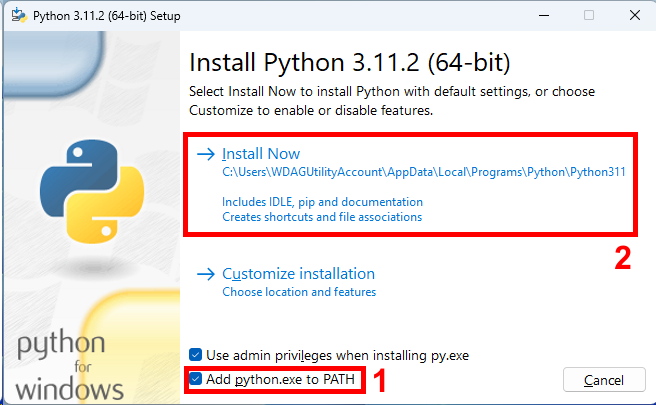
\includegraphics[width=0.495\linewidth]{PythonInstallPath.png}
        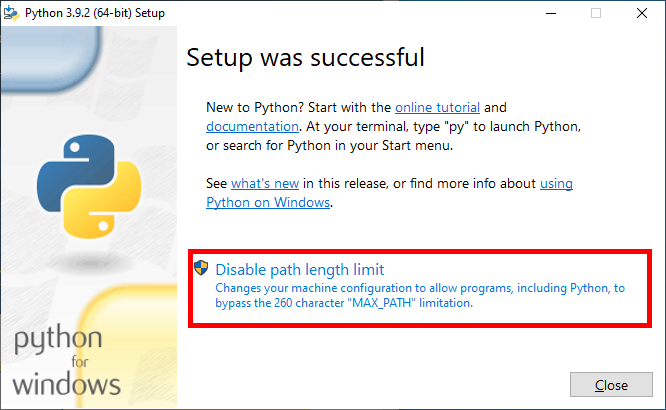
\includegraphics[width=0.495\linewidth]{PythonInstallPathLimit.png}
    \end{center}
    Pro ověření instalace napíšeme v příkazové řádce příkaz \code{python}.\footnote{Na počítačích s Linuxem je příkaz v terminálu \code{python3}.}
    Tím se spustí \abbreviation{REPL}\footnote{{\bf R}ead-{\bf E}valuate-{\bf P}rint-{\bf L}oop.} Pythonu, ve které můžeme již psát všechny příkazy programovacího jazyka, které se po zadání ihned provedou a vypíšou výsledek.

\subsubsection{Instalace doplňujících knihoven}
\label{sec:pip}
    Samotná instalace Pythonu obsahuje jen minimální množství nejnutnějších knihoven.
    My budeme využívat ještě následující rozšiřující knihovny:
    \begin{itemize}
        \item \file{\href{https://numpy.org}{NumPy}} ({\bf Num}erical {\bf Py}thon: numerická matematika, řady a vícedimenzionální datové typy),
        \item \file{\href{https://scipy.org}{SciPy}} ({\bf Sci}entific {\bf Py}thon: algoritmy pro optimalizaci, statistiku, řešení diferenciálních rovnic, lineární algebru, atd.),
        \item \file{\href{https://matplotlib.org}{Matplotlib}} (vizualizace, grafy).
    \end{itemize}
    K jejich doinstalování slouží modul \code{pip}.
    V příkazové řádce napíšeme
    \begin{lstlisting}
        python -m pip install numpy scipy matplotlib\end{lstlisting}
    čímž se nainstalují naráz všechny tři knihovny.\footnote{
        Pokud na počítači s Linuxem uvedený postup nebude fungovat, je potřeba nejprve nainstalovat instalátor \file{pip} pomocí příkazu \code{sudo apt install python3-pip}.
        Pak lze použít buď výše uvedený příkaz, nebo stručnější \code{pip3 install numpy}.
    }
    
    Existuje samozřejmě celá řada dalších užitečných a používaných knihoven, jako je například \file{\href{https://pandas.pydata.org/}{Pandas}} pro analýzu dat nebo \file{\href{https://www.sympy.org/}{SymPy}} pro symbolické výpočty, na které v tomto kurzu nedojde.

\subsection{Instalace Visual Studio Code}
    Instalace jazyka Python obsahuje jednoduché vývojové prostředí nazvané \abbreviation{\href{https://docs.python.org/3/library/idle.html}{IDLE}}.\footnote{
        {\bf I}ntegrated {\bf D}evelopment and {\bf L}earning {\bf E}nvironment.
    }
    To však poskytuje jen omezené možnosti co se týče ladění, psaní rozsáhlejších projektů s více zdrojovými soubory nebo integrace s verzovacími programy.

    Pro serióznější práci budeme používat \href{https://code.visualstudio.com}{Visual Studio Code} s doplňkem pro programovací jazyk Python.
    Instalační soubor stáhnete ze stránky \href{https://code.visualstudio.com}{code.visualstudio.com}.
    Během instalace na počítač s Windows doporučuji zvolit obě možnosti \uv{Add Open with Code action to...},
    \begin{center}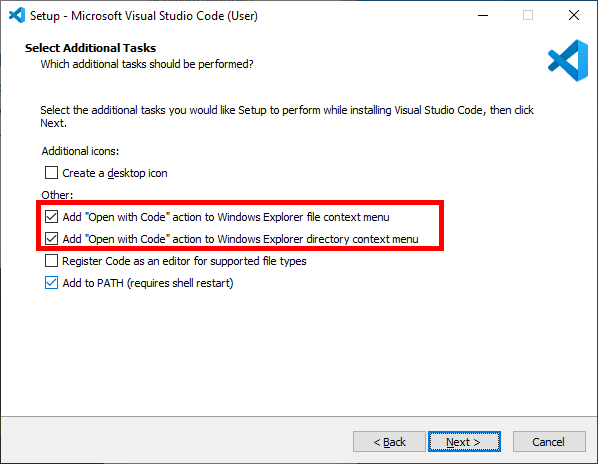
\includegraphics[width=0.5\linewidth]{VSCodeInstall.png}\end{center}
    což zjednoduší otevírání složek s projekty nebo samostatných souborů pomocí pravého tlačítka myši.

    Na operačním systému Linux je nejjednodušší provést instalci pomocí Snap Store příkazem v terminálu
    \begin{lstlisting}
        sudo snap install --classic code\end{lstlisting}
    nebo použít tento \href{https://code.visualstudio.com/docs/setup/linux}{návod}.

\subsubsection{Instalace doplňku pro Python}
    \begin{center}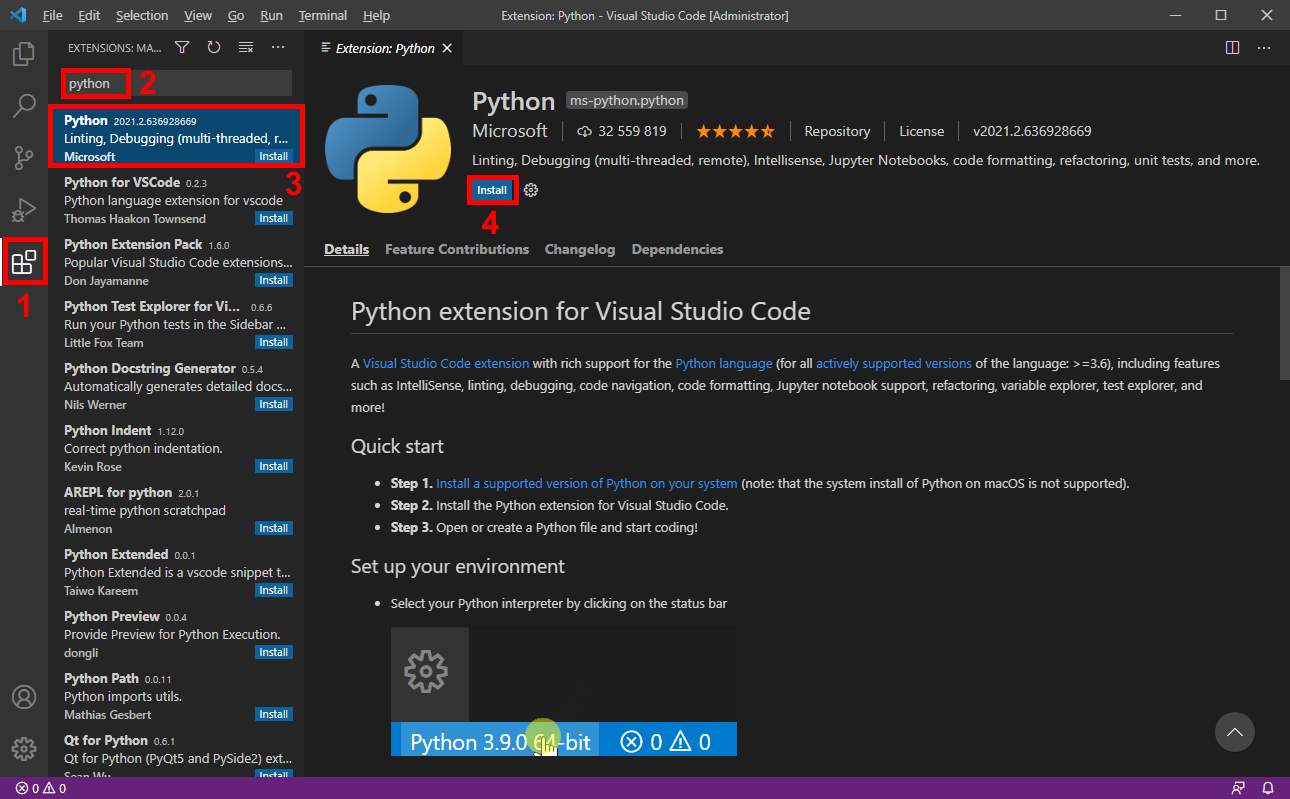
\includegraphics[width=\linewidth]{VSCodeInstallPython.png}\end{center}
    Ke správě doplňků (extensions) se dostanete kliknutím na ikonku {\color{red} 1} nebo stisknutím \code{Ctrl+Shift+X}. 
    Vyhledáte doplněk \href{https://marketplace.visualstudio.com/items?itemName=ms-python.python}{Python} {\color{red} 2} od Microsoftu, vyberete ho {\color{red} 3} a nainstalujete {\color{red} 4}.

\subsection{Instalace Git}
    Instalační soubor verzovacího systému \href{https://git-scm.com}{Git} stáhnete z webové stránky \href{https://git-scm.com}{git-scm.com}.
    K instalaci Gitu potřebujete administrátorská práva.
    
    V následujícím postupu zobrazuji jen ty snímky obrazovky, na kterých je vhodné vybrat jinou volbu, než jaká je instalátorem standardně nabízena.
    \begin{center}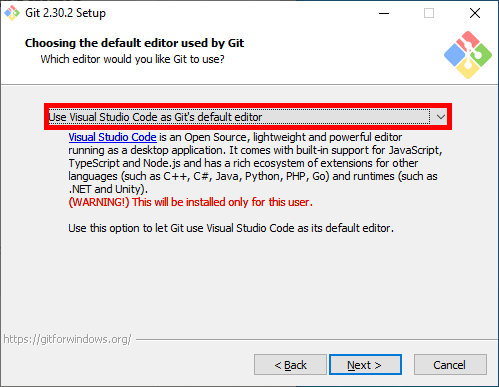
\includegraphics[width=0.5\linewidth]{GitInstallEditor.png}\end{center}
    Jako editor zvolíme dříve nainstalované Visual Studio Code.
    Systém Git vyžaduje editor jednak pro povinný komentář každé zapsané změny (commit), jednak pro ošetření kolizí při slučování větví (merge).
    \begin{center}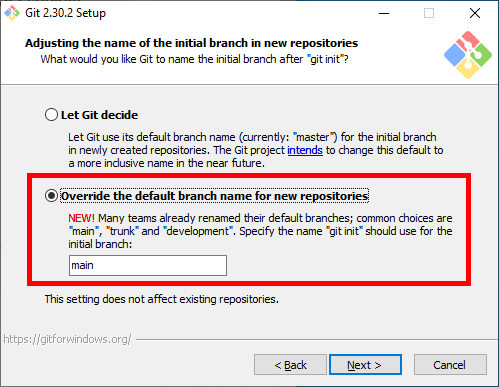
\includegraphics[width=0.5\linewidth]{GitInstallMain.png}\end{center}
    Hlavní větev repozitáře se donedávna standardně jmenovala \code{master}.
    Vzhledem k negativním konotacím tohoto slova v angličtině se přechází na neutrálnější označení.
    Nejběžnější je \code{main}, na které již přešel i populární správce vzdálených repozitářů \href{https://github.com}{GitHub}.
    Doporučuji tedy zvolit pojmenování \code{main}.

    Všechna nastavení lze samozřejmě kdykoliv po instalaci změnit.

\section{Úvod do používaných nástrojů}
    V této sekci naleznete základy použití verzovacího systému Git a úvod do syntaxe a idiomatiky jazyka Python.
    Na rozdíl od zbytku poznámek bude tato sekce v průběhu cvičení postupně doplňována podle toho, s jakými technikami se seznámíme v hlavní části cvičení.

\subsection{Verzovací systém Git}
    Každý si patrně už někdy v životě zasteskl, že nemá uložené dřívější verze svých souborů.
    Změny, které se ukazují být nevhodné či provedené omylem (kočka nepozorovaně přejde po klávesnici a my pak soubor uložíme), kamarád, který z nějakých důvodů chce tu verzi vašeho programu, kterou jste mu poskytli před rokem, a vy jste mezitím kód zásadně přepsali, to vše jsou důvody k předsevzetí nějakým způsobem důležité milníky v práci na projektu archivovat.

    Triviální verzování může spočívat například v ručním ukládání kopií projektu s daty či jinými označeními jednotlivých verzí.
    Takovýto postup je ale velmi těžkopádný, jelikož v každé kopii musí být uloženy všechny soubory projektu, i pokud se v nich od předchozí verze nic nezměnilo.
    Obtížně se vyhledává, co přesně se mezi jednotlivými verzemi změnilo a kdo změnu provedl, pokud na projektu pracuje větší tým, přičemž obtížnost roste s velikostí a komplexností projektu.
    Pro usnadnění uchovávání historie změn proto vznikly verzovací systémy.    

    Verzovací systém pomáhá udržet historii změn souborů projektu, přičemž ke každému snímku historie se lze vrátit.
    Vše provádí chytře a v maximální míře automaticky.
    Systém sám sleduje, v jakých souborech byly provedeny změny.
    Pokud se jedná o textový soubor, umí porovnat aktuální a libovolnou historickou verzi řádek po řádku a zvýraznit odlišnosti.
    Umožňuje pracovat s nezávislými vývojovými větvemi (\emph{branches}), ve kterých lze například zkoušet různý přístup k řešení daného problému a mezi kterými lze jednoduše přepínat.
    Vybrané řešení lze pak snadno začlenit (\emph{merge}) do hlavní vývojové větve.

    Soubory projektu a informace o jejich historických změnách se nazývá souhrnně \emph{repozitář}.
    V něm se uchovávají nejen verze souborů, ale také údaje o tom, kdo a kdy změny provedl.
    To předurčuje verzovací systémy pro efektivní správu týmových projektů, kdy každý člen týmu pracuje na určité části projektu a své změny následně do projektu včleňuje.

    My budeme používat verzovací systém \href{https://git-scm.com}{Git}.
    Ten patří mezi \emph{distribuované} verzovací systémy\footnote{
        Další distribuované verzovací systémy jsou například \href{https://www.mercurial-scm.org/}{Mercurial}, \href{https://bazaar.canonical.com}{Bazaar} či \href{http://darcs.net/}{Darcs}.
    }, což znamená, že každý uživatel má na svém počítači celý obsah repozitáře a pouze ve chvílích, kdy uzná za vhodné nebo kdy je k tomu příležitost, může své změny synchronizovat se \emph{vzdáleným repozitářem}, ve kterém se shromažďují změny od všech členů týmu, začleňují do hlavní vývojové větve projektu a hlídají případné kolize.
    Výhody tohoto přístupu oproti centralizovaným verzovacím systémům\footnote{
        Nejznámější reprezentant centralizovaného verzovacího systému je \href{https://subversion.apache.org/}{Subversion}.
    } jsou následující:
    \begin{enumerate}
        \item Práce na projektu nevyžaduje připojení k nějakému centrálnímu serveru s repozitářem, a tedy můžete pracovat offline klidně někdě v džungli nebo na Marsu.
        \item Není potřeba spravovat zvlášť server s repozitářem a zvlášť klientské počítače. Vše je na jednom místě.
        \item Při práci na týmovém projektu není případná porucha počítače spojená se ztrátou dat žádná katastrofa, protože ostatní kolegové mají celou kopii repozitáře na svých počítačích.
    \end{enumerate}
    Git nejefektivněji funguje na textové soubory, ale zvládne verzovat i soubory binární (například obrázky).

    Git je v dnešní době jeden z nejpopulárnějších verzovacích systémů.
    Pod jedho správou jsou vyvíjeny i velké projekty, například samo \href{https://github.com/microsoft/vscode}{Visual Studio Code}.
    Tento projekt je navíc otevřený (open source), což znamená, že kdokoliv, tedy i vy nebo já, má přístup k celému repozitáři, tedy ke všem zdrojovým kódům a k jejich kompletní historii. 
    Může se do práce na projektu zapojit, přispět k jeho vývoji a začít psát historii sám.
    
    Program Git pochází z prostředí Linuxu a je navržený tak, aby se s ním dalo pracovat z příkazové řádky (terminálu) pomocí jednoduchých textových příkazů.
    Tímto způsobem lze používat všechny dostupné funkce Gitu.
    My se s nejdůležitějšími funkcemi seznámíme právě pomocí textových příkazů, protože na nich se nejlépe naučí, jak tento Git funguje a jaké jsou jeho možnosti.
    Jakmile si člověk ujasní principy verzování pomocí Gitu, může využít některý z množství nástrojů a doplňků pro různé programy, které práci s repozitáři usnadní a zrychlí.
    Obsluha Git repozitářů je integrována i do vývojového prostředí Visual Studio Code.

    Na stránkách projektu Git najdete \href{https://git-scm.com/book/en/v2}{podrobný interaktivní návod} ke všem funkcím verzovacího systému (a to částečně i v \href{https://git-scm.com/book/cs/v2}{češtině}).

\subsubsection{Prvotní nastavení}
    Git nelze používat do té doby, než jsou nastaveny základní informace o uživateli.
    To se provede pomocí příkazů v příkazové řádce (terminálu)
    \begin{lstlisting}
        git config --global user.name "..."
        git config --global user.email "..."\end{lstlisting}
    přičemž za ... doplníte své jméno (přezdívku) a email.
    Těmito údaji se podepisují všechny zapsané změny v repozitáři.
    Pokud tedy spolupracujete na projektu s jinými lidmi, je dobré zvolit takové údaje, pomocí kterých vás kolegové snadno identifikují a úspěšně kontaktují.

    Výpis všech nastavení získáte příkazem
    \begin{lstlisting}
        git config --list\end{lstlisting}
    Uvidíte, že v mezi nastaveními je i název hlavní větve repozitáře (\code{init.defaultbranch=main}) a cesta k nastavenému textovému editoru (v našem případě Visual Studio Code).

    Všechna nastavení a práci s příkazem \code{config} najdete v tomto \href{https://git-scm.com/docs/git-config}{podrobném návodu} nebo zadáním příkazu
    \begin{lstlisting}
        git help config\end{lstlisting}

\subsubsection{Čtyři možné stavy souborů v repozitáři}
    \begin{itemize}
        \item \emph{Nesledovaný (untracked):} 
            Systém Git historii tohoto souboru neuchovává.
            Každý nové vytvořený soubor je v tomto stavu.
            Speciální podskupinu tvoří \emph{ignorované (ignored)} soubory, což bývají v drtivé většině pomocné soubory nebo soubory s citlivými údaji.
            Seznam ignorovaných souborů se uvede do speciálního souboru \file{.gitignore}, o kterém pojednává sekce~\ref{sec:gitignore}.

        \item \emph{Připravený k zapsání (staged):} 
            Soubor je systémem Git sledován (verzován).
            Od předchozího zapsání v něm došlo ke změnám (nebo byl nově vytvořen) a k zapsání byl připraven pomocí příkazu
            \begin{lstlisting}
        git add soubor\end{lstlisting}
            Hromadný příkaz
            \begin{lstlisting}
        git add *\end{lstlisting}
            připraví k zapsání všechny změněné soubory a všechny nové soubory kromě těch, které jsou uvedeny v souboru \file{.gitignore} (viz sekce~\ref{sec:gitignore}).

            Přehled změn v souborech připravených k zapsání oproti naposledy uložené verzi dá příkaz
            \begin{lstlisting}
        git diff --staged\end{lstlisting}

            Verze souborů se změnami připravenými k zapsání jsou uloženy mimo pracovní adresář: při dodatečných modifikacích souboru se k těmto verzím souboru lze vrátit příkazem
            \begin{lstlisting}
        git restore --staged soubor\end{lstlisting}
            (pozor, tímto příkazem se nenávratně ztratí všechny změny v souboru, které byly provedeny od jeho poslední přípravy k zapsání).

        \item \emph{Změněný (modified):} 
            Soubor je systémem Git sledován (verzován).
            Od předchozího zapsání v něm došlo ke změnám, avšak soubor ještě nebyl označen k zapsání.
            Přehled změn v souborech oproti naposledy uložené verzi či oproti verzi připravené k zapsání dá příkaz
            \begin{lstlisting}
        git diff\end{lstlisting}
        
        \item \emph{Zapsaný (committed):} 
            Soubor je systémem Git sledován (verzován) a jeho historie je zaznamenána v repozitáři.
            Jedná se o verzi souboru, ke které je vždy možné se vrátit.
            Zapsání (commit) všech souborů připravených k zapsání (staged) se provede příkazem
            \begin{lstlisting}
        git commit [m "popis revize"]\end{lstlisting}
            kde \code{"popis revize"} je povinné označení ukládaného historického snímku.
            Pokud se neuvede část v hranatých závorkách, systém Git spustí textový editor zvolený při jeho instalaci a v něm otevře soubor, do kterého název revize a případně nějaké podrobnější komentáře uvedete.
            Po uložení souboru a uzavření textového editoru se provede zapsání.
    \end{itemize}

\subsubsection{Životní cyklus souborů v repozitáři}
Práci s repozitářem budu demonstrovat na příkladu projektu pro integraci diferenciálních rovnic ze sekce~\ref{sec:ODR1}.

\subsubsubsection{Vytvoření nového repozitáře}
    Ve složce, jejíž historii chceme ukládat, se repozitář vytvoří jednoduchým příkazem
    \begin{lstlisting}
        git init\end{lstlisting}
    Existenci repozitáře lze vždy odhalit pomocí skryté podsložky s názvem \code{.git}:
    \begin{center}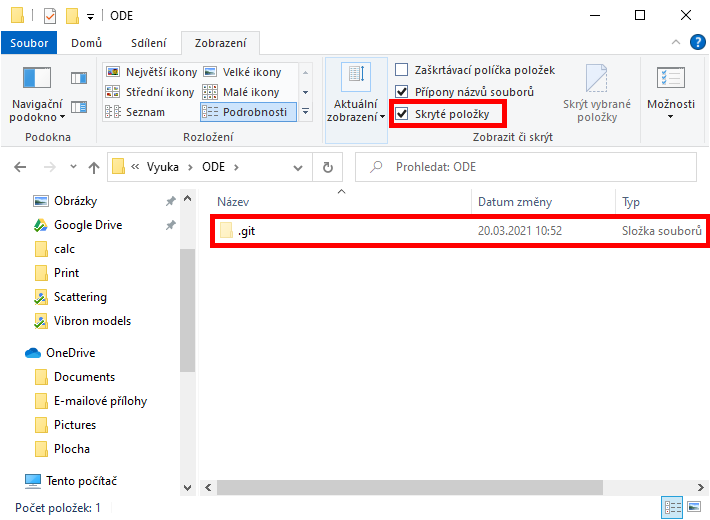
\includegraphics[width=0.7\linewidth]{FolderGit.png}\end{center}
    V této složce je uložena veškerá zapsaná historie vašeho projektu od jeho vytvoření.
    Pokud tuto složku smažete, přijdete tím o \uv{paměť} systému Git pro daný projekt, avšak aktuální soubory projektu zůstanou tak, jak jsou.
    Pokud naopak přesunete nebo překopírujete složku s projektem včetně podsložky \code{.git} kamkoliv jinam, klidně na jiný počítač, kopírujete zároveň celou historii projektu.
    Nedoporučuji jakkoliv měnit soubory v této složce, protože tím můžete nevratně narušit integritu repozitáře a systém Git přestane být schopen repozítář používat.

\subsubsubsection{Stav repozitáře}
    Aktuální stav repozitáře kdykoliv zjistíte pomocí
    \begin{lstlisting}
        git status\end{lstlisting}
    Příkaz vypíše název aktuální větve a stav všech souborů v projektu.
    Pro čerstvě vytvořený repozitář se dozvíte něco takového:
    \begin{center}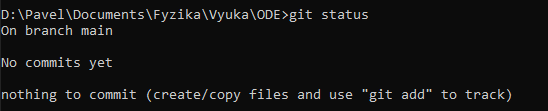
\includegraphics[width=0.6\linewidth]{GitStatusEmpty.png}\end{center}

\subsubsubsection{Vytvoření a první zapsání nového souboru}
    Ve složce s projektem otevřeme Visual Studio Code (napsáním \code{code} do příkazové řádky nebo stiskem pravého tlačítka myši nad otevřenou složkou a výběrem \uv{Open with Code}), vytvoříme nový soubor a uložíme ho jako \file{ode.py}.
    Příkaz \code{git status} ukáže
    \begin{center}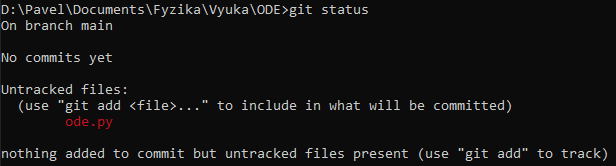
\includegraphics[width=0.7\linewidth]{GitStatusFirst.png}\end{center}
    Systém Git si je vědom toho, že si uživatel nemusí pamatovat všechny příkazy, a proto se snaží práci usnadnit a napovídá, které další akce lze v další fázi použít a jak.

    Příkazem \code{git add *} se nový soubor připraví k zapsání.
    Stav repozitáře se změní takto:
    \begin{center}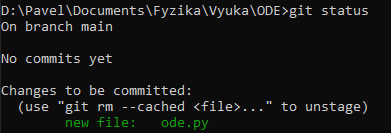
\includegraphics[width=0.45\linewidth]{GitStatusAdd.png}\end{center}

    Zapsání se provede příkazem \code{git commit}.
    Otevře se editor (nový soubor ve Visual Studiu Code), do kterého uvedeme stručný a výstižný popis změn:
    \begin{center}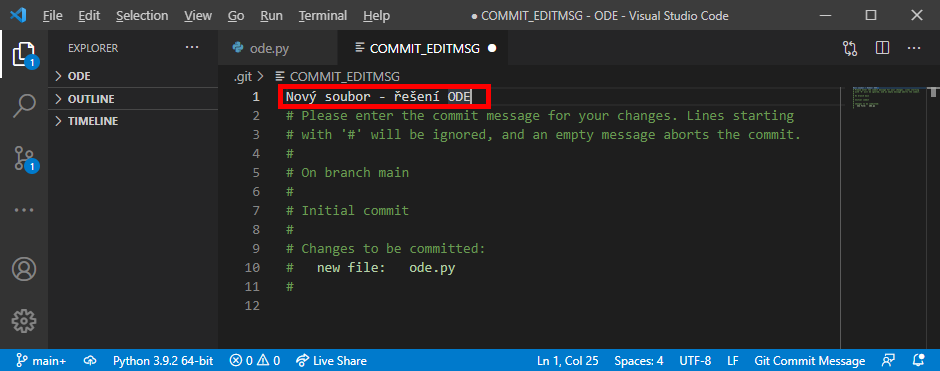
\includegraphics[width=0.9\linewidth]{VSCodeCommit.png}\end{center}
    Po uložení a zavření souboru se vytvoří první snímek historie našeho projektu.
    V příkazové řádce vidíme stručný souhrn, co se zapsalo.
    \begin{center}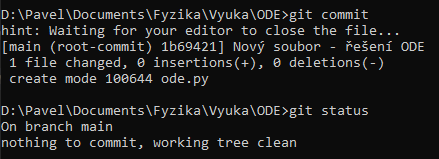
\includegraphics[width=0.5\linewidth]{GitStatusCommit.png}\end{center}

\subsubsubsection{Změny v souboru}
    Do souboru \file{ode.py} vepíšeme první část kódu, kterým bude řešení jedné diferenciální rovnice Eulerovou metodou 1. řádu.

    \begin{lstlisting}[style=TinyPython]
        def euler_1(model, y, t, dt):
            y1 = y + model(y, t) * dt
            t1 = t + dt
            return y1, t1
        
        def ode_solve(model, initial_condition, integrator=runge_kutta_4, dt=0.1, maxt=10):
            y = initial_condition                   # Initial conditions
            ys = [y]                                # List with results
            
            t = 0                                   # Actual time
            ts = [t]                                # List with times
            
            while t < maxt:
                y, t = integrator(model, y, t, dt)  # Step
                
                ys.append(y)                        # Store position
                ts.append(t)                        # Store time
                    
            return ys, ts
        
        def relaxation(y, t):
            return -y
        
        ys, ts = ode_solve(relaxation, 1)\end{lstlisting}
    Po spuštění kód vyřeší diferenciální rovnici relaxace~\eqref{eq:relaxace} a v proměnných \code{ys} a \code{ts} vrátí seznam $y$-ových hodnot a odpovídajících časových okamžiků $t$.

    Kód funguje a dává smysluplné výsledky ($y(t)$ klesá s rostoucím časem k nule), zapíšeme tedy změny do \uv{historie}.
    Stav repozitáře je
    \begin{center}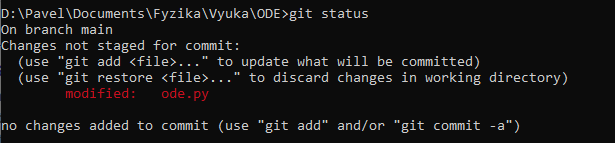
\includegraphics[width=0.7\linewidth]{GitStatusChange.png}\end{center}
    Soubor je ve stavu změněný (modified).
    Před zapsáním je nutné jeho stav změnit na k zapsání (staged) pomocí příkazu \code{git add *}.
    Lze také použít zkrácený příkaz
    \begin{lstlisting}
        git commit -a\end{lstlisting}
    který všechny změněné soubory převede do stavu k zapsání a rovnou zapsání provede.
    Změnu označním popisem \uv{Eulerova metoda 1. řádu}.
    \begin{center}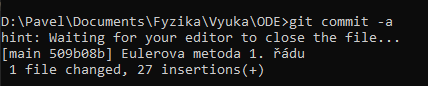
\includegraphics[width=0.5\linewidth]{GitStatusCommit2.png}\end{center}

    {\color{blue} Dobrá programátorská praxe je zapisovat vždy jen takový kód, který lze spustit, tj. který neobsahuje žádné syntaktické chyby.}

\subsubsubsection{Přidání dalšího souboru do projektu}
    V programu na řešení diferenciálních rovnic je dobré oddělit univerzální výpočetní funkce od funkcí specifických pro daný model.
    Vytvoříme tedy nový soubor \file{relaxation.py}, do kterého přesuneme kód
    \begin{lstlisting}[style=TinyPython]
        import ode

        def relaxation(y, t):
            return -y
        
        ys, ts = ode.ode_solve(relaxation, 1)\end{lstlisting}
    Nesmíme zapomenout náš \uv{modul} naimportovat pomocí příkazu \code{import ode}.
    Program lze spustit a funguje, je tedy dobrý čas tyto změny zapsat.
    Nejdříve se ale podíváme na stav repozitáře:    
    \begin{center}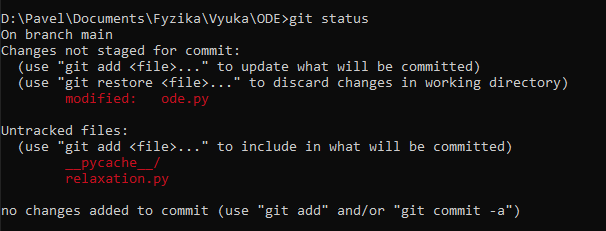
\includegraphics[width=0.7\linewidth]{GitStatusChange2.png}\end{center}
    Soubor \file{ode.py} se změnil, soubor \file{relaxation.py} byl vytvořen a zatím je ve stavu nesledován.
    Navíc se ještě vytvořila celá složka \file{__pycache__/}.\footnote{
        Pro urychlení provádění celého programu ukládá do tohoto adresáře interpret Pythonu speciálně předpřipravené používané moduly.
    }
    Jedná se o pomocnou složku, kterou verzovat nechceme.
    Toho se docílí buď tím, že ji ponecháme v nesledovaném stavu (untracked) a začneme sledovat jen nový soubor.
    Tento postup však znemožní používání hromadných příkazů \code{git add *} či \code{git commit -a}.
    Gitu lze speciálně naznačit, jaké soubory a jaké složky jsou jen pomocné, a má je tedy ignorovat.
    Za tím účelem se vytvoří speciální soubor pojmenovaný \file{.gitignore}, do kterého zapíšeme následující pravidlo
    \begin{lstlisting}
        __pycache__/\end{lstlisting}
    a uložíme.
    Stav repozitáře se změní následovně:
    \begin{center}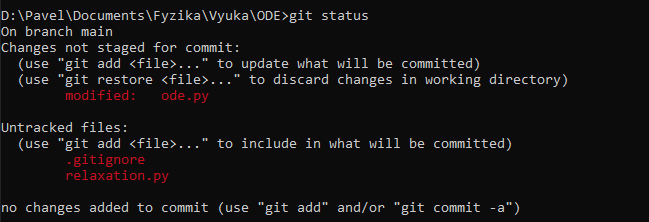
\includegraphics[width=0.7\linewidth]{GitStatusIgnore.png}\end{center}
    Pomocná složka už není uvedena mezi nesledovanými soubory a Git ji ignoruje.
    Můžeme již připravit k zapsání všechny nové a změněné soubory pomocí hromadného příkazu \code{git add *} a následně zapsat všechny změn pomocí \code{git commit},
    přičemž změnu pojmenuji \uv{Oddělení řešitele ODE a modelu}.

\subsubsubsection{Zobrazení historie revizí}
\label{sec:gitlog}
    Historie zobrazíme příkazem
    \begin{lstlisting}
        git log\end{lstlisting}
    \begin{center}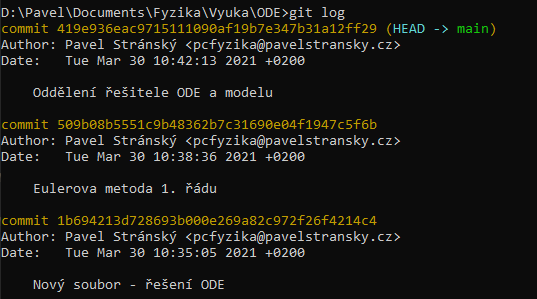
\includegraphics[width=0.7\linewidth]{GitLog.png}\end{center}
    Vypsaný seznam obsahuje všechny údaje o jednotlivých snímcích historie (zapsáních), tj. datum a čas, autora a jeho e-mail a hash kód podepisující zapsání.

    Příkaz log má velké možnosti, jak formátovat a filtrovat informace o zapsáních, přičemž všechny jsou uvedeny v \href{https://git-scm.com/docs/git-log}{referenční příručce}.
    Nejdůležitější jsou
    \begin{itemize}
        \item \code{git log -{}-oneline} naformátuje vše hezčím způsobem (každé zapsání na jednom řádku) a z hashe zobrazí jen prvních 7 znaků, což stačí k identifikaci jednotlivých zapsání,
        \item \code{git log -2} vypíše jen poslední dva záznamy,
        \item \code{git log -{}-stat} vypíše statistiky o jednotlivých verzích (počty změn a výpis změněných souborů),
        \item \code{git log -{}-graph} zobrazí výsledek \uv{graficky}, což se hodí v případě více větví (větve budou vysvětleny v sekci~\ref{sec:branches}),
        \item \code{git log -{}-follow ode.py} vypíše všechny historické změny v souboru \file{ode.py},
        \item \code{git log -{}-since "2 years 1 day 3 minutes ago"} 
        \item \code{git log -{}-until "2019-01-15"} vypíše všechny změny od, resp. do uvedeného časového údaje,
        \item \code{git log -{}-author="Pavel"} vypíše všechny změny, které zapsal uživatel Pavel,
        \item \code{git log -{}-grep="Euler"} vypíše všechny změny, které obsahují v popisu slovo \uv{Euler}.
    \end{itemize}
    Uvedené filtry lze samozřejmě libovolně kombinovat.

\subsubsection{.gitignore}
\label{sec:gitignore}
    Překladače programovacích jazyků často vytvářejí v adresáři projektu dočasné pomocné soubory, které nechcete, aby se staly součástí repozitáře (tyto soubory nenesou žádnou relevantní informaci, navíc mohou na různých počítačích vypadat jinak podle toho, jaký překladač či jaké vývojové prostředí zrovna použijete).
    Abyste mohli používat příkazy pro hromadné sledování či zapisování souborů \code{git add *} či \code{git commit -a}, musíte GITu naznačit, jaké soubory má ignorovat.
    K tomu slouží soubor \code{.gitignore}.
    
    Každé pravidlo v souboru \code{.gitignore} zabírá jeden řádek.
    Řádek, který začíná znakem \#, je ignorován a může sloužit například jako komentář.
    Příklady jednotlivých řádků:
    \begin{itemize}
    \item \code{tajne.txt}
        
        Ignoruje soubor s názvem \code{tajne.txt} (může obsahovat třeba přihlašovací údaje k nějaké službě a ty rozhodně nechceme sdílet ani archivovat; nezapomeňte, že co je jednou zapsané v repozitáři, z něj až na výjimky nelze odstranit).

    \item \code{*.log}
    
        Ignoruje všechny soubory s příponou \code{log},

    \item \code{!important.log}

        ale neignoruje soubor \code{important.log}.

    \item \code{*.[oa]}

        Ignoruje všechny soubory s příponou \code{o} nebo \code{a}.

    \item \code{temp/}

        Ignoruje všechny soubory v podadresáři \code{temp}.

    \item \code{doc/**/*.pdf}
    
        Ignoruje všechny soubory s příponou \code{pdf} v podadresáři \code{doc} a ve všech jeho podadresářích.
        Neignoruje však soubory s příponou \code{pdf} v hlavním adresáři projektu.
    \end{itemize}
    Další příklady jsou například~\href{https://www.atlassian.com/git/tutorials/saving-changes/gitignore}{zde}.

    Pokud na GitHubu zakládáte nový projekt, můžete upřesnit, jaký programovací jazyk budete používat a GitHub automaticky vytvoří optimální soubor \code{.gitignore}.

    \begin{voluntary}
        Podívejte se do souboru \ghfile{}{.gitignore} v repozitáři k těmto zápiskům.
        Zatímco Python si téměř žádné pomocné soubory nevytváří, {\LaTeX} jich generuje požehnaně.
        Proto je tento soubor celkem dlouhý. 
    \end{voluntary}

\subsubsection{Větve}
\label{sec:branches}
    Verzovací systém Git umožňuje pracovat paralelně na několika různých verzích kódu a mezi nimi dokáže efektivně přepínat.
    Větvení se hodí v případě, že chceme vyzkoušet více různých přístupů k řešení úlohy.
    Pro každé vytvoříme vlastní větev úprav, což dovolí řešení porovnávat a nakonec vybrat to, které vyhovuje nejvíce.
    Každou větev můžeme dále větvit.
    Perspektivní větve lze následně slučovat dohromady, neperspektivní lze nechat být.
    
    Častá programátorská praxe je taková, že v hlavní větvi\footnote{Hlavní větev se donedávna pojmenovávala \code{master}, dnes se spíše prosazuje pojmenování \code{main}.} se nachází vždy jen odladěná a otestovaná verze programu.
    Pro každou změnu v projektu se vytvoří nová větev.
    Na té se může pracovat hodinu, ale třeba několik měsíců.
    V této \uv{vývojové} větvi se změny provedou, odladí, pošlou testerům, a teprve poté se začlení do hlavní větve.
    Mezitím je stále k dispozici funkční program hlavní větve, který lze bez obav používat k ostrému provozu.

\subsubsubsection{Vytvoření nové větve}
    Budeme pokračovat ve vývoji programu pro řešení obyčejných diferenciálních rovnic.
    Předpokládejme, že řešení pro jednu rovnici máme hotové a chceme ho rozšířit tak, bych fungovalo i na soustavu více diferenciálních rovnic 1. řádu, kterým se věnuje sekce~\ref{sec:ODRn}.
    K tomu vytvoříme novou větev \code{odesystem}
    \begin{lstlisting}
        git branch odesystem\end{lstlisting}
    a přepneme se na ni příkazem\footnote{
        Vytvoření nové větve a přepnutí se do ní lze jedním příkazem \code{git switch -c odesystem}.
    }
    \begin{lstlisting}
        git switch odesystem\end{lstlisting}
        Zpět na hlavní větev se lze vrátit příkazem \code{git switch main}.\footnote{
            Git umožňuje přepínání mezi větvemi také pomocí příkazu \code{git checkout}.
        }

\subsubsubsection{Výpis větví}
    Seznam všech větví se vypíše příkazem
    \begin{lstlisting}
        git branch\end{lstlisting}
    \begin{center}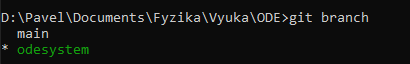
\includegraphics[width=0.45\linewidth]{GitBranch.png}\end{center}
    Aktivní větev je vyznačena hvězdičkou i barevně.

    Další užitečná upřesnění výpisu větví jsou
    \begin{itemize}
        \item \code{git branch -{}-merged} vypíše jen větve spojené s aktuální větví,
        \item \code{git branch -{}-no-merged} vypíše jen větve nespojené s aktuální větví.
    \end{itemize}

\subsubsubsection{Změny a sloučení větví}
    Poté, co provedeme a odladíme změny související s rozšířením programu na výpočet soustavy diferenciálních rovnic ve větvi \code{odesystem}, můžeme tyto změny začlenit do hlavní větve \code{main}.
    K tomu slouží příkaz
    \begin{lstlisting}
        git merge odesystem\end{lstlisting}
    spuštěný v hlavní větvi.
    Pokud během slučování nedojde k žádným konfliktům, vše proběhne hladce.
    Může se však stát, že byly provedeny změny na stejném místě jednoho souboru v obou větvích (konflikt).
    V tom případě Git označí konflikty v souborech a jejich stav změní na modifikovaný.
    Pak je potřeba tyto soubory projít, vybrat z konfliktních verzí jednu, případně kód upravit tak, aby odrážel obě konfliktní změny, a zapsat příkazem \code{git commit -a}.
    Tím je slučování dokončeno.    
    
\subsubsubsection{Odstranění větve}
    Větev odstraníme prostým
    \begin{lstlisting}
        git branch -d odesystem\end{lstlisting}
    Odstraňovat větve má smysl jen v případě, kdy jsme přesvědčeni, že změny v ní provedené byla slepá cesta.

\subsubsection{Návrat k dřívějším verzím}
    Pozor, při neopatrném použití těchto příkazů hrozí ztráta dat!
    Pokud si budete následující příkazy zkoušet, doporučuji vám zazálohovat si celou složku s projektem včetně repozitáře (složky \file{.git}).

    \begin{itemize}
        \item \code{git commit -{}-amend} umožňuje změnit popis posledního zapsání.
        \item \code{git restore soubor} vrátí změny uvedeného souboru na posledně zapsanou verzi (lze použít i hromadné \code{git restore *}\footnote{\code{git restore *} se chová podobně jako \code{git reset -{}-hard}.}).
        \item \code{git reset HEAD\~{}1} zruší poslední\footnote{Číslo udává, o kolik revizí se vracíme zpět.} zapsání, avšak soubory ve složce projektu ponechá tak, jak jsou.\footnote{HEAD vlastně značí ukazatel na poslední zapsání.}
        \item \code{git reset -{}-hard HEAD\~{}1} zruší poslední zapsání a soubory projektu uvede do stavu, v jakém byly na začátku této poslední revize. 
        Všechny provedené změny jsou nenávratně ztraceny.
        Pokud byl nějaký soubor v poslední revizi vytvořen, je smazán.
        Toto je nejnebezpečnější příkaz, proto používejte jen v opravdu odůvodněných případech.
        \item \code{git reset 946cb25} se vrátí na zapsání, jehož hash začíná uvedeným číslem.
        \item \code{git reset ORIG_HEAD} se vrátí na tu zapsanou verzi, na které jsme byli bezprostředně před použitím posledního příkazu \code{git reset}.
        \item \code{git checkout -b oldrev 946cb25} vytvoří novou větev nazvanou \uv{oldrev}, ve které budou soubory ve stavu, kdy bylo provedeno zapsání s uvedeným hashem (hash zjistíme například pomocí \code{git log -{}-oneline} popsaného v sekci~\ref{sec:gitlog}).
        \item \code{git checkout 946cb25} vrátí se do tohoto zapsání, ale ponechá historii tak, jak je.\footnote{Tzv. Detached HEAD state.}.
            K návratu zpět stačí použít příkaz pro přepnutí do hlavní větve \code{git switch main}.
    \end{itemize}

\subsubsection{Vzdálené repozitáře}\label{sec:GITRemote}
    Verzovací systém GIT umí kromě sledování a uchovávání historie změn souborů vašeho projektu i koordinovat změny, které provádí na projektu více řešitelů (pracovní tým). 
    K tomu slouží vzdálené repozitáře.
    Mezi nejrozšířenější systémy patří
    \begin{itemize}
    \item \href{https://github.com}{GitHub}: 
        Na něm si každý může zdarma zřídit vlastní repozitáře a používat je například k~synchronizaci svého projektu mezi různými počítači, pro sdílení vlastních výtvorů s komunitou nebo právě pro spolupráci ve vlastním týmu. 
        Vlastníkem firmy vyvíjející tento systém je Microsoft.
        Z toho důvodu je základní práce s ním integrována i co vývojového prostředí Visual Studio Code.
    \item \href{https://gitlab.mff.cuni.cz}{GitLab}: 
        Open source řešení, základní verze rovněž zdarma, k pokročilé verzi má MFF UK licenci.
    \end{itemize}
    Oba systémy disponují webovým rozhraním, ze kterého lze projekty jednoduše spravovat, a~rovněž desktopovými aplikacemi, které umožňují pracovat s lokálními repozitáři pomocí jednoduchého rozhraní.
    Pro GitHub existuje například \href{https://desktop.github.com}{GitHub Desktop}.
    Projekty mohou být soukromé (přístup k nim máte pouze vy či ti, kterým pošlete pozvánku) nebo veřejné (přístup má kdokoliv).

    Tyto zápisky a vzorové ukázky kódů jsou veřejně na GitHubu a můžete k nim dostat na adrese \url{https://github.com/PavelStransky/PCInPhysics2021}.
    K dispozici je samozřejmě celý repozitář s historií se všemi commity a se všemi vývojovými větvemi.
    Repozitář můžete stáhnout buď z uvedené webové stránky (zelené tlačítko \code{Clone or download}), nebo pomocí programu git.

    \begin{itemize}
    \item \code{git clone https://github.com/PavelStransky/PCInPhysics2021}
    
        V aktuální složce vytvoří podsložku \code{PCInPhysics} a do ní stáhne celý repozitář.
        V případě těchto zápisků se jedná o tento soubor v {\LaTeX}u,
        výsledné PDF, EPS či PNG verze všech obrázků a všechny zdrojové kódy.

    \item \code{git remote -v}
    
        V adresáři s lokálním repozitářem ukáže, na jaký vzdálený repozitář je navázaný.
        Stejně jako základní větev se standardně jmenuje \code{main}, vzdálený repozitář se standardně jmenuje \code{origin}.
        Vy můžete mít na jeden projekt navázáno více vzdálených repozitářů, každý pak samozřejmě musíte pojmenovat jinak.

    \item \code{git remote add origin https://github.com/Uzivatel/VzdalenyRepozitar}
    
        Přidá do vašeho projektu odkaz na vzdálený repozitář umístěný na GitHubu.

    \item \code{git remote show origin}
    
        Zobrazí informace o vzdáleném repozitáři.

    \item \code{git pull}
    
        Do adresáře s lokálním repozitářem stáhne aktuální verzi aktuální větve.
        Pokud máte lokálně rozpracované změny, stažení se nepovede.
        Pokud máte uložené změny (commit), git se automaticky pokusí vaše změny sloučit se změnami v globálním repozitáři (merge).
        
    \item \code{git fetch}
    
        Stáhne celý vzdálený repozitář (všechny větve).
    
    \item \code{git push origin master}
    
        Do vzdáleného repozitáře \code{origin} zapíše vaši větev \code{master}.
        Vzdálený repozitář může být nastaven tak, že vaše změny musí ještě někdo schválit.

    \item \code{git push}

        Zkrácený zápis, pokud jste dříve nastavili pomocí příkazu \code{git push --set-upstream origin master} název lokální větve a příslušného vzdáleného repozitáře.

    \end{itemize}

    Další informace najdete například v \href{https://git-scm.com/book/cs/v2/Z%C3%A1klady-pr%C3%A1ce-se-syst%C3%A9mem-Git-Pr%C3%A1ce-se-vzd%C3%A1len%C3%BDmi-repozit%C3%A1%C5%99i}{dokumentaci}.

    \begin{task}
        Stáhněte si do svých počítačů (naklonujte si) z GitHubu repozitář s poznámkami k tomuto cvičení.
        V budoucnu si pomocí příkazu \code{git pull} stahujte aktuální verze.
        Můžete si vytvořit pracovní větev poznámek a v ní si s kódy hrát.
        V hlavní větvi \code{master} se vám uchová originální verze ze~vzdáleného repozitáře.
    \end{task}

    \begin{task}
        Vytvořte si účet na GitHubu, vytvořte prázdný projekt a navažte si ho s dříve na cvičení vytvořeným lokálním repozitářem pomocí příkazů \code{git remote add} (plný příkaz výše).
        Následně si do vzdáleného repozitáře nahrajte lokální repozitář pomocí příkazu \code{git push}. 
    \end{task}

\subsubsection{Cheat Sheet}
    Pro snadnou orientaci v použití Gitu bez nutnosti pamatovat si všechny příkazy je dostupný \href{https://training.github.com/downloads/github-git-cheat-sheet.pdf}{Git Cheat Sheet} nebo \href{https://ndpsoftware.com/git-cheatsheet.html}{tento interaktivní web}.

\subsection{Programovací jazyk Python}
    Python je v dnešní době velmi populární programovací jazyk, který pronikl do spousty rozmanitých odvětví, a to zejména díky bohatosti a pokročilosti knihoven, které jsou vyvíjeny komunitou a jsou díky tomu aktuální a odladěné (či průběžně odlaďované).
    Python existuje na mnoha platformách od osobních počítačů po mikrokontroléry a dá se v něm naprogramovat téměř cokoliv: pokročilé vědecké výpočty používající nejnovější numerické algoritmy, dobře vypadající grafy, statistická analýza, analýza velkých dat a strojové učení, ale také webové služby, okénkové programy či editace obrázků a videí.
    Je běžné, že i komerční programy obsahují Python coby skriptovací jazyk, čímž umožňují uživateli používat své vlastní kódy \uv{uvnitř} komerčního produktu a integrovat různé programy mezi sebou.\footnote{
        Jako příklad poslouží nejnovější verze programu \href{https://www.wolfram.com/language/12/external-system-integration/evaluate-python-in-a-notebook.html}{Mathematica}, \href{https://www.originlab.com/doc/python/Run-Python-in-Origin}{Origin} či \href{https://developer.sas.com/guides/python.html}{SAS}.
    }
    
    Python lze charakterizovat jako jazyk:
    \begin{itemize}
        \item 
            \emph{Interpetovaný}, což znamená, že provádění programů probíhá přímo ze zdrojového kódu.\footnote{
                Mezi další známé interpetované jazyky patří napříkad JavaScript nebo PHP.
            }
            Ke spouštění kódů je tedy potřeba mít nainstalovaný interpret, což jsme učinili v sekci~\ref{sec:InstalacePython}.
            Pokud kód obsahuje syntaktickou chybu, je odhalena až ve chvíli, kdy se na ni interpret při provádění kódu narazí.
            U interpretovaných jazyků se neztrácí čas překladem do strojového kódu a je pro ně přirozené dynamické typování proměnných.
            Tím, že interpet čte text kódu příkaz po příkazu, je provádění programů pomalejší, ale vzhledem k tomu, že velká část časově náročných funkcí a knihoven bývá napsána v rychlejších programovacích jazycích, není to zásadní nevýhoda.
            
            Opakem intepretovaných jazyků jsou jazyky kompilované, přičemž kompilace se provádí buď přímo do strojového kódu daného procesoru\footnote{Například C/C++, Pascal nebo Fortran.} nebo do mezikódu. Ten  ke spuštění vyžaduje dodatečnou kompilaci, která však může být vysoce optimalizovaná přímo pro danou hardwarovou konfiguraci použitého počítače.\footnote{Zde se jedná napřílad o jazyky Java, C\# a celý .NET framework nebo Julia.}

        \item 
            \emph{Dynamicky typovaný}, což znamená, že proměnná nemusí mít předem daný typ a typ proměnné se může za běhu programu dokonce měnit.
        
        \item 
            \emph{S automatickou správou paměti}, takže programátor se nemusí starat o alokování a uvolňování paměti. 
            Python při inicializaci proměnné paměť alokuje automaticky a ve chvíli, kdy proměnnou přestaneme používat, paměť uvolní.\footnote{Algoritmus se nazývá \emph{Garbage collection}.} 

        \item
            V Pythonu lze pythonovským způsobem používat tři základní programovací paradigmata: \emph{procedurální, objektové a funkcionální}.
    \end{itemize}
         
    Python klade důraz na jednoduchost, stručnost a čitelnost kódu.
    Filosofie programovacího jazyka je shrnuta v \href{https://www.python.org/dev/peps/pep-0020/}{Zenu Pythonu},\footnote{
        Zen se také vypíše, pokud do svého kódu zadáte \code{import this}.
    } se kterým vám doporučuji se seznámit.

\subsubsection{Vytvoření a spuštění kódu}
    Ve Visual Studio Code vytvoříme nový soubor a uložíme si ho s příponou \code{*.py}. 
    Podle této přípony VS Code pozná, že se jedná o pythonovský kód a použije k práci s ním správný doplněk.
       
    Hotový kód lze spustit ve VS Code jedním z následujících tří způsobů.
    \begin{enumerate}
        \item 
            \emph{Kliknutím na zelenou šipku na nástrojové liště}:
            Tímto způsobem se spustí celý soubor kódu.
        \item
            \emph{Stiskem \code{F5}} (a výběrem Python File): Kód se spustí v režimu ladění (debugger).
            Zastaví se na každém kontrolním bodě (breakpoint, který se vloží na vybranou řádku kódu klávesou \code{F9}) nebo na každé chybě.
            Pro pokračování provádění kódu stačí stisknout buď znovu \code{F5}, nebo \code{F10} či \code{F11} pro jeden krok.

        \item
            \emph{Označením části kódu a stiskem Ctrl+Enter}: V okně \code{TERMINAL} spustí \abbreviation{REPL} Pythonu a v něm označenou část kódu.
            \abbreviation{REPL} se po provedení kódu nezavře, takže v něm lze psát dodatečné příkazy.
            Pro ukončení \abbreviation{REPL} do něj stačí napsat \code{exit()} nebo v něm stisknout \code{Ctrl+Z} a potvrdit.
            \abbreviation{REPL} musí být ukončen, než se použije jakákoliv z dvou dříve popsaných metod spuštění kódu.
    \end{enumerate}

\subsubsection{Základy syntaxe Pythonu}
    Soubor se vzorovými příklady najdete v repozitáři ke cvičení: \ghfile{python/basics/}{introduction.py}.\footnote{
        Vzorový soubor je inspirován příkladem \href{https://learnxinyminutes.com/docs/cs-cz/python/}{Nauč se Python v Y minutách}.
    }
    Doporučuji vám si ho stáhnout nebo jeho obsah překopírovat a důsledně si ho řádek po řádku projít a spouštět nejlépe pomocí označení a stiskem \code{Ctrl+Enter}, jak bylo popsáno v předchozí sekci.
    Některé části kódu odkazují na proměnné zavedené v dřívější části souboru, proto kód procházejte postupně od začátku do konce.

    Z vzorového kódu bych vypíchl následující body:
    \begin{enumerate}
        \item 
            \emph{Základní datové typy a operátory}: Zaměřte se na možnosti formátování řetězců. 
            Python obsahuje jen dva základní číselné typy: \code{int} a \code{float}.
            Zbytek je podobný jako v jiných programovacích jazycích.

        \item
            \emph{Proměnné a kolekce}: 
            Důležité standardní kolekce jsou \emph{seznam} (list) [...] a \emph{slovník} (dicctionary) \{...\}.
            Dále existuje typ \emph{n-tice} (tuple) (...) a \emph{množina} (set) \{...\}.
            O jaký typ kolekce se jedná poznáte podle typu závorek, kterými je uzavřena.
            Python nabízí bohaté možnosti indexování prvků kolekcí.

            Python nemá typ \uv{řada} (jedno či vícerozměrný soubor hodnot stejných typů).
            Ten je implementován až v rozšiřujících knihovnách, například v knihovně \file{numpy}, které se budeme věnovat později.
            
        \item
            \emph{Podmínky a cykly}:
            Příkaz uvozující blok kódu vždy končí znakem \uv{:}.
            Každý blok je definován svým odsazením, které musí být na každém řádku stejné
            (tj. musí obsahovat stejný počet odsazujících znaků, mezi které patří buď mezera nebo tabulátor).
            Konvence je používat k odsazení \href{https://www.python.org/dev/peps/pep-0008/#indentation}{4 mezery}.

            Cykly jsou možné pouze přes iterovatelné objekty.
            Pro cyklus přes přirozená čísla (indexy) musíme vytvořit odpovídající iterovatelný objekt příkazem \code{range}.
            V drtivé většině se lze při programování v Pythonu indexům zcela vyhnout.

        \item 
            \emph{Funkce}: Python umožnuje velkou variabilitu co se týče argumentů funkce a návratových hodnot díky své funkci automatického sbalení a rozbalení kolekcí.
            Funkce se navíc chová jako objekt, lze ji tedy přiřadit jakékoliv proměnné.
            To je jeden z prvků funkcionálního programování.

            Funkcionální programování také obsahuje koncept anonymní funkce, což je jednoduchá funkce definovaná na jednom řádku, která nemá vlastní jméno.
            V Pythonu se vytváří pomocí klíčového slova \code{lambda}.

        \item 
            \emph{Moduly}: Při programování je důležité vhodně strukturovat kód.
            Python obsahuje jednoduchý koncept modulů, přičemž každý soubor s příponou \code{*.py} lze použít jako modul.
            Modul je vlastně speciální typ objektu.

            Dobře se seznamte se způsoby, jak modul načíst a používat, jelikož většina funkcí Pythonu se nachází právě v modulech.
            Jedná se například o matematické funkce v modulu \file{math} nebo rozšiřující knihovny \file{numpy}, \file{scipy} a \file{matplotlib}.

        \item 
            \emph{Třídy}: Python umožňuje objektově orientované programování.
            Práce s třídami se však v mnohém liší od striktně objektově orientovaných programovacích jazyků, jakými jsou například C++, C\# nebo Java.
            Důležitý rozdíl je například v přístupnosti atributů (všechny atributy v Pythonu jsou veřejné).
            Rovněž dědičnost a dědění metod se chová odlišně.
            Dále je nutné pamatovat na to, že každá metoda třídy musí mít v deklaraci jako první argument odkaz na instanci, se kterou je volána (konvenčně se označuje \code{self}).
            Ve vzorovém kódu je k objektovému programování opravdu jen to nejnutnější minimum.
            Pokud chcete v Pythonu využívat objekty seriózně, doporučuji pročíst si odpovídající \href{https://docs.python.org/3/tutorial/classes.html}{kapitolu v manuálu}.
    \end{enumerate}

    Uvedený kód s příklady obsahuje jen ty struktury jazyka Python, které budeme používat.
    V budoucích cvičeních se ještě seznámíte se \emph{správou kontextu} (klíčové slovo \code{with}).
    Python umožňuje navíc 
    \begin{itemize}
        \item ošetření chyb pomocí \emph{výjimek} (klíčová slova \code{raise}, \code{try}, \code{except}, \code{finally}),
        \item tvorbu \emph{generátorů} (klíčové slovo \code{yield}),
        \item \emph{asynchronní programování}, korutiny a úkoly (klíčová slova \code{await}, \code{async})
        \item či tvorbu a použití \emph{dekorátorů}.
    \end{itemize}
    Pro plné ovládnutí jazyka vám doporučuji se v budoucnu s těmito koncepty seznámit, a to buď ze specializovaných přednášek, z tutoriálů a návodů na webu, nebo studiem cizích kódů.

    Na oficiálních stránkách Pythonu najdete \href{https://docs.python.org/3/tutorial/}{tutoriál k nejnovější verzi programovacího jazyka}.

\subsubsection{Pojmenování proměnných a formátování}
    Formátování kódu Pythonu je celkem volné.
    Povinné je dodržet jen správné odsazení bloků.
    Pro snazší čitelnost kódu byla nicméně vytvořena řada doporučení, která najdete souhrnně na stránce \href{https://www.python.org/dev/peps/pep-0008}{PEP 8}.\footnote{\abbreviation{PEP} = {\bf P}ython {\bf E}nhancement {\bf P}roposal}
    Python obsahuje dokonce knihovnu \file{\href{https://pypi.org/project/autopep8/}{autopep8}}, která váš zdrojový soubor podle těchto pravidel naformátuje.
    Automatické formátování podle PEP 8 lze nastavit i ve \href{https://code.visualstudio.com/docs/python/editing#_formatting}{Visual Studiu Code}.
        
    Pro pojmenování proměnných existuje jediné závazné pravidlo, které zní, že indentifikátor se nesmí shodovat s žádným z \href{https://docs.python.org/3/reference/lexical_analysis.html#keywords}{35 klíčových slov} jazyka.
    Kromě toho jsou ve výše uvedeném dokumentu další nezávazná pravidla k pojmenování proměnných:\footnote{
        Čitelnosti různých stylů pojmenování proměnných se věnují i seriózní vědecké články, například
        \url{http://www.cs.kent.edu/~jmaletic/papers/ICPC2010-CamelCaseUnderScoreClouds.pdf}.
    }
    \begin{itemize}
        \item
            \emph{Proměnné a funkce} se doporučuje pojmenovávat malými písmeny a jednotlivá slova spojovat podtržítky, tzv. underscore style (například \code{pocet_bodu}).
        \item
            \emph{Konstanty} se doporučuje pojmenovávat velkými písmeny a jednotlivá slova spojovat podtržítky (například \code{PLANCKOVA_KONSTANTA}).
        \item
            \emph{Třídy} se doporučuje pojmenovávat tak, že jednotlivá slova názvu začínají velkým písmenem a mezi nimi není žádný znak, tzv. Pascal style (například \code{PostovniAdresa}).
        \item
            \emph{Moduly} se doporučuje pojmenovávat krátkými výstižnými názvy složenými jen z malých písmen.
        \item
            Kvůli čitelnosti je dobré se vyhnout jednopísmenným označením \code{l}, \code{I} a \code{O}, jelikož takto označené proměnné mohou být snadno zaměněny s čísly \code{1} a \code{0}.

    \end{itemize}
    Pokud vám vyhovuje jiný styl pojmenovávání, lze ho použít.
    Je však dobré být v pojmenovávání konzistentní napříč celým projektem.

    Častá otázka je, zda proměnné označovat \emph{česky či anglicky}.
    Jelikož nikdy nevíte, kdo v dnešním propojeném světě bude chtít váš kód použít a třeba i upravit pro své potřeby, doporučuji používat anglická pojmenování.
    
    Snadná čitelnost kódu je podpořena i vhodným psaním \emph{komentářů}.
    Na drouhou stranu je vhodné vycházet z předpokladu, že dobře napsaný kód je čitelný i bez komentářů.
    Čitelnost totiž zaručují zejména vhodně a výstižně označené proměnné a správně navržená struktura kódu.
    Komentovat je dobré jen ty části kódu, kde se používá nějaký ne všeobecně známý trik nebo postup.
    Nadbytek komentářů je velmi těžké udržovat při úpravách a může vést i k tomu, že po několika změnách kódu nebudou komentáře v souladu s tím, co kód vykonává.
    
    Naopak doporučené je nešetřit popisem, co dělají jednotlivé funkce, jaké jsou jejich argumenty a co vracejí na výstupu.
    K tomu slouží komentář typu \emph{docstring}, který je vysvětlený v souboru \ghfile{python/basics/}{introduction.py} v sekci o funkcích.\footnote{
        Stejně jako v mluvených jazycích se zlepšujete čtením literatury, v programovacích jazycích pomáhá čtení cizích kódů.
        Pro přiklad použití komentářů se koukněte třeba na zdrojový soubor funkce \code{\href{https://github.com/scipy/scipy/blob/master/scipy/optimize/optimize.py}{optimize}} z knihovny \file{scipy}.
    }
    Použití \emph{docstringu} usnadní i tvorbu a správu doprovodné dokumentace k celému projektu.
    Existují například nástroje, které vám z těchto komentářů vytvoří strukturované webové stránky.

\subsubsection{Řady (knihovna numpy)}
\label{sec:numpy}
    Jak bylo zmíněno v předchozí sekci, definice jazyka Python neobsahuje typ \emph{řada}, tj. jedno či vícerozměrně pole hodnot stejného typu.

    Základy práce s řadami jsou vysvětleny přímo v souboru \ghfile{python/basics/}{arrays.py} v repozitáři.

\subsubsection{Grafy (knihovna matplotlib)}
    K vykreslení grafů slouží knihovna \file{\href{https://matplotlib.org}{Matplotlib}}.
    V základní instalaci Pythonu není obsažena, je nutné ji doinstalovat podle návodu v sekci~\ref{sec:pip}.

    Jednoduchý příklad vykreslení grafů je v souboru \ghfile{python/basics/}{plot.py} v repozitáři.

\subsubsection{Pseudonáhodná čísla}\label{sec:PseudonahodnaCisla}
    V Pythonu lze pseudonáhodná čísla generovat pomocí několika knihoven.
    \begin{itemize}
        \item 
            Pro základní použití je k dispozici knihovna \file{\href{https://docs.python.org/3/library/random.html}{random}}.
            Z ní nejdůležitější funkce jsou tyto:
            \begin{itemize}
                \item \code{random()}: \emph{reálné} pseudonáhodné číslo $x$ rovnoměrně z intervalu $x\in\langle 0;1)$.
                \item \code{uniform(a, b)}: \emph{reálné} pseudonáhodné číslo $x$ rovnoměrně z intervalu $x\in\langle a;b\rangle$.
                \item \code{gauss(mu, sigma)}: pseudonáhodné číslo z Gaussovského rozdělení se střední hodnotou \code{mu} a směrodatnou odchylkou \code{sigma}. 
                \item \code{randint(a, b)}: \emph{celé} pseudonáhodné číslo $d$ z intervalu $a\leq d<b$.
                \item \code{seed(s)}: nastaví počáteční násadu generátoru podle parametru \code{s} (pro jednu konkrétní násadu bude generátor dávat stejnou sekvenci čísel). 
                Parametr může být jakéhokoliv typu, tedy číslo, řetězec atd. 
                Pokud se parametr neuvede, použije se jako násada systémový čas.
                \item \code{choice(l)}: vybere pseudonáhodně element ze seznamu \code{l}.
                \item \code{shuffle(l)}: promíchá elementy v seznamu \code{l}.
            \end{itemize}

        \item
            Ke generování řad či vícerozměrných objektů, jejichž elementy jsou náhodná čísla, lze použít i knihovnu \file{numpy}, viz sekce~\ref{sec:numpy} a soubor s příklady~\ghfile{python/basics/}{numpy.py}.

        \item 
            Pro pokročilejší použití je knihovna \file{\href{https://numpy.org/doc/stable/reference/random/index.html}{numpy.random}}.
            Ta umožňuje zvolit vlastní generátor pseudonáhodných čísel, generovat čísla z celé řady \href{https://numpy.org/doc/stable/reference/random/generator.html}{statistických rozdělení} a generovat naráz celé vektory či matice.
            \begin{itemize}
                \item \code{generator = default_rng()}: Inicializuje standardní generátor pseudonáhodných čísel.
                \item \code{generator = Generator(PCG64())}: Inicializuje specifický generátor pseudonáhodných čísel (v~tomto případě PCG-64, což je O'Neillův permutační kongruenční generátor).
                \item \code{generator.random(size=10)}: vektor délky 10 s elementy z rovnoměrného rozdělení z~intervalu $\langle 0;1)$.
                \item \code{generator.normal(size=10)}: vektor délky 10 s elementy z normálního Gaussova rozdělení se střední hodnotou $0$ a směrodatnou odchylkou $1$.
                \item \code{generator.normal(loc=1, scale=2, size=(10,10))}: matice rozměru $10\times10$ s elementy z normálního Gaussova rozdělení se střední hodnotou $1$ a směrodatnou odchylkou $2$.
            \end{itemize}            
    \end{itemize}


\section{Obyčejné diferenciální rovnice 1. řádu}
\label{sec:ODR1}
    V této části se budeme věnovat řešení jedné diferenciální rovnice prvního řádu,
    \begin{equation}
        \derivative{y}{t}=f(y,t)
    \end{equation}
    s počáteční podmínkou
    \begin{equation}
        y(t_{0})=y_{0}.
    \end{equation}
    Zde $y=y(t)$ je hledaná funkce a $t$ je nezávisle proměnná.
    
    Numerické řešení diferenciální rovnice spočívá v nahrazení infinitezimálních přírůstků přírůstky konečnými:
    \begin{equation}\label{eq:Diference}
        \frac{\Delta y}{\Delta t}=\phi(y,t)
    \end{equation}
    kde $\phi$ je funkce, která udává směr, podél kterého se při numerickém řešení vydáme.
    Volbá této funkce je klíčová a záleží na ní, jak přesné řešení dostaneme a jak rychle ho dostaneme.

\subsection{Pár důležitých pojmů}
    \begin{itemize}
        \item{\bf Explicitní algoritmy:}
        K výpočtu hodnoty funkce $y_{i+1}$ se vyžadují pouze hodnoty z aktuálních a minulých kroků, tj. $y_{i}$, $y_{i-1}$, atd.

        \item {\bf Jednokrokové algoritmy:}
        K výpočtu hodnoty funkce $y_{i+1}$ v následujícím kroku vyžadují pouze znalost hodnoty funkce v aktuálním kroku $y_{i}$.
        Rozepsáním~\eqref{eq:Diference} dostaneme
        \begin{equation}
            \label{eq:phi}
            \boxed{
                y_{i+1}=y_{i}+\underbrace{\phi(y_{i},t_{i})}_{\phi_{i}}\Delta t
            },
        \end{equation}
        přičemž počáteční hodnota $y_{0}$ je dána počáteční podmínkou.
        My se omezíme pouze na tyto algoritmy.

        \item {\bf Lokální diskretizační chyba:}
        \begin{equation}
            \mathcal{L}=y(t+\Delta t)-y(t)-\phi(y(t),t)\Delta t,
        \end{equation}        
        kde $y(t)$ udává přesné řešení v čase $t$.

        \item {\bf Akumulovaná diskretizační chyba:}
        \begin{equation}
            \label{eq:AkumulovanaChyba}
            \epsilon_{i}=y_{i}-y(t_{i})
        \end{equation}

        \item {\bf Řád metody:} 
        Metoda je $p$-tého řádu, pokud
        \begin{equation}\label{eq:RadMetodyODR}
            L(\Delta t)=\mathcal{O}(\Delta t^{p+1}).
        \end{equation}

        \item {\bf Kontrola chyby řešení:}
        Chybu numerického řešení diferenciální rovnice lze zmenšit 1)~menším krokem, 2)~lepší metodou (metodou vyššího řádu). 
        Menší krok však znamená vyšší výpočetní čas.
        Sofistikované metody proto průběžně mění velikost kroku: když se funkce mění pomalu, krok prodlouží, když se mění rychle, krok zkrátí (tzv. {\bf metody s adaptivním krokem}).
        Tím se docílí vysoké přesnosti při co nejmenším výpočetním čase.
    \end{itemize}

\subsection{Eulerova metoda 1. řádu}
    \begin{equation}\label{eq:Euler1}
        \phi_{i}=f(y_{i},t_{i}),
    \end{equation}
    tj. krok do $y_{i+1}$ děláme vždy ve směru tečny v bodě $y_{i}$.

    \begin{itemize}
        \item Nejjednodušší metoda integrace diferenciálních rovnic.
        \item Chyba je obrovská, k dosažení přesných hodnot je potřeba velmi malého kroku, což znamená dlouhý výpočetní čas.
    \end{itemize}

\subsection{Eulerova metoda 2. řádu}
    \begin{align}\label{eq:Euler2a}
        k_{1}&=f(y_{i},t_{i})\nonumber\\
        k_{2}&=f\left(y_{i}+k_{1}\Delta t,t+\Delta t\right)\\
        \phi_{i}&=\frac{1}{2}\left(k_{1}+k_{2}\right),\nonumber
    \end{align}
    tj. uděláme jednoduchý Eulerův krok ve směru $k_{1}$, spočítáme derivaci $k_{2}$ po tomto kroku a vyrazíme z bodu $y_{i}$ ve směru, který je průměrem obou směrů (doporučuji si nakreslit obrázek).

    Ekvivalentní je udělat \uv{Eulerův půlkrok} a vyrazit z bodu $y_{i}$ ve směru derivace spočtené po~tomto půlkroku:
    \begin{align}\label{eq:Euler2b}
        k'_{1}&=f(y_{i},t_{i})\nonumber\\
        k'_{2}&=f\left(y_{i}+k'_{1}\frac{\Delta t}{2},t+\frac{\Delta t}{2}\right)\\
        \phi_{i}&=k'_{2}\nonumber
    \end{align}

\subsection{Runge-Kuttova metoda 4. řádu}
    \begin{align}\label{eq:RungeKutta}
        k_{1}&=f(y_{i},t_{i})\nonumber\\
        k_{2}&=f\left(y_{i}+k_{1}\frac{\Delta t}{2},t+\frac{\Delta t}{2}\right)\nonumber\\
        k_{3}&=f\left(y_{i}+k_{2}\frac{\Delta t}{2},t+\frac{\Delta t}{2}\right)\\
        k_{4}&=f\left(y_{i}+k_{3}\Delta t,t+\Delta t\right)\nonumber\\
        \phi_{i}&=\frac{1}{6}\left(k_{1}+2k_{2}+2k_{3}+k_{4}\right)\nonumber
    \end{align}
    
    \begin{itemize}
        \item Jedna z nejčastěji používaných metod.
        \item Vysoká rychlost a přesnost při relativní jednoduchosti.
        \item Existují i Runge-Kuttovy metody vyššího řádu $p$, avšak vyžadují výpočet více než $p$ dílčích derivací $k_{j}$.
        Obecně platí, že metoda řádu $p\leq4$ vyžaduje $p$ derivací, metoda řádu $5\leq p\leq7$ vyžaduje $p+1$ derivací a metoda řádu $p=8,9$ vyřaduje $p+2$ derivací.
    \end{itemize}

\subsection{Odvození metod}
    Metody se odvozují na základě rozvoje do Taylorovy řady.
    Volně řečeno platí, že kolik členů Taylorova rozvoje se vezme, takový bude řád metody $p$.

    \begin{itemize}
        \item \emph{Eulerova metoda 1. řádu.} Odvození je triviální:
            \begin{equation}
                y(t+\Delta t)\approx y(t)+\underbrace{y'(t)}_{f(y,t)}\Delta t,
            \end{equation}
            takže
            \begin{equation}
                y_{i+1}=y_{i}+f(y_{i},t_{i})\Delta t.
            \end{equation}
        \item \emph{Eulerova metoda 2. řádu.}
            \begin{align}
                y(t+\Delta t)
                    &\approx y(t)+y'(t)\Delta t+\frac{1}{2}\underbrace{y''(t)}_{\approx\frac{y'(t+\Delta t)-y'(t)}{\Delta t}}\Delta t^{2}\nonumber\\
                    &\approx y(t)+f(y,t)\Delta t+\frac{1}{2}[f(\underbrace{y(t+\Delta t)}_{\approx y(t)+y'(t)\Delta t},t+\Delta t)-f(y,t)]\Delta t\nonumber\\
                    &\approx y(t)+\frac{1}{2}\left[f(y,t)+f(y(t)+f(y,t)\Delta t,t+\Delta t)\right]\Delta t,
            \end{align}
            a odtud
            \begin{equation}
                y_{i+1}=y_{i}+\underbrace{\frac{1}{2}\left[f(y_{i},t_{i})+f(y_{i}+f(y_{i},t_{i})\Delta t,t_{i+1})\right]}_{\phi_{i}}\Delta t,
            \end{equation}
            což je jen jinak napsané vztahy~\eqref{eq:Euler2a}.

            Druhá Eulerova metoda 2. řádu~\eqref{eq:Euler2b} se obdrží stejným způsobem, jen při aproximaci druhé derivace se použije poloviční krok:
            \begin{equation}
                y''(t)\approx\frac{y'\left(t+\frac{\Delta t}{2}\right)-y'(t)}{\frac{\Delta t}{2}}.
            \end{equation}

            \begin{voluntary}
                Dokončete odvození vztahů~\eqref{eq:Euler2b}.
            \end{voluntary}            
    \end{itemize}

    Analogicky se postupuje při odvození metod vyššího řádu.
    Jeho složitost však narůstá exponenciálně s řádem metody.
    U Eulerovy metody 2. řádu se navíc ukázalo, že lze odvodit několik stejně dobrých vztahů.
    Tato volnost s řádem metody narůstá.

\newpage
\subsection{Domácí úkol na 23.3.2021}
\begin{task}
\label{task:ODR1}
    Naprogramujte Eulerovu metodu 1. a 2. řádu a Runge-Kuttovu metodu.
    Vyřešte numericky diferenciální relaxační rovnici\footnote{
        Rovnice popisuje například Newtonův zákon chladnutí tělesa, aktuální množství prvku při radioaktivním rozpadu nebo různé populační modely.
    }
    \begin{equation}\label{eq:relaxace}
        \derivative{y}{t}=-y
    \end{equation}
    s počátečními podmínkami $y_{0}=1$ (analytickým řešením je funkce $e^{-t}$).
    Integrační krok $\Delta t$ ponechte jako volný parametr.
    Nakreslete grafy řešení $y(t)$ pro rozdílné hodnoty integračních kroků, například $\Delta t=0.01$ a $\Delta t=0.1$ pro čas $t\in\langle0;10\rangle$.
\end{task}

\setcounter{solution}{1}
\begin{solution}
    \label{sol:ODR1}
    Jedno možné řešení v souborech \ghfile{python/ode/}{ode.py} (integrační metoda), \ghfile{python/ode/}{graphs.py} (vykreslování grafů) a \ghfile{python/ode/}{relaxation.py} (hlavní soubor, který obsahuje definici modelu a volá všechny výpočetní a vykreslovací funkce).
    Na řešení této úlohy je také ukázán základ práce s větvemi v sekci~\ref{sec:branches}.
    
    \begin{figure}[!htbp]
        \begin{subfigure}{0.49\linewidth}
            \centering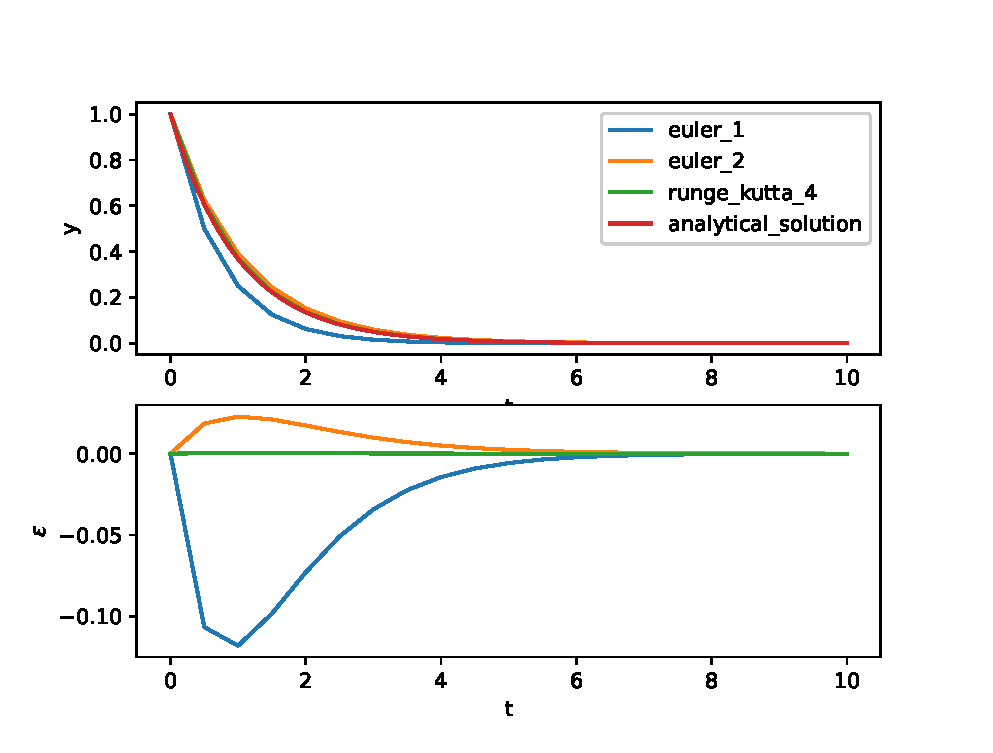
\epsfig{file=relaxation_methods.eps,width=\linewidth}
        \end{subfigure}
        \hfill
        \begin{subfigure}{0.49\linewidth}
            \centering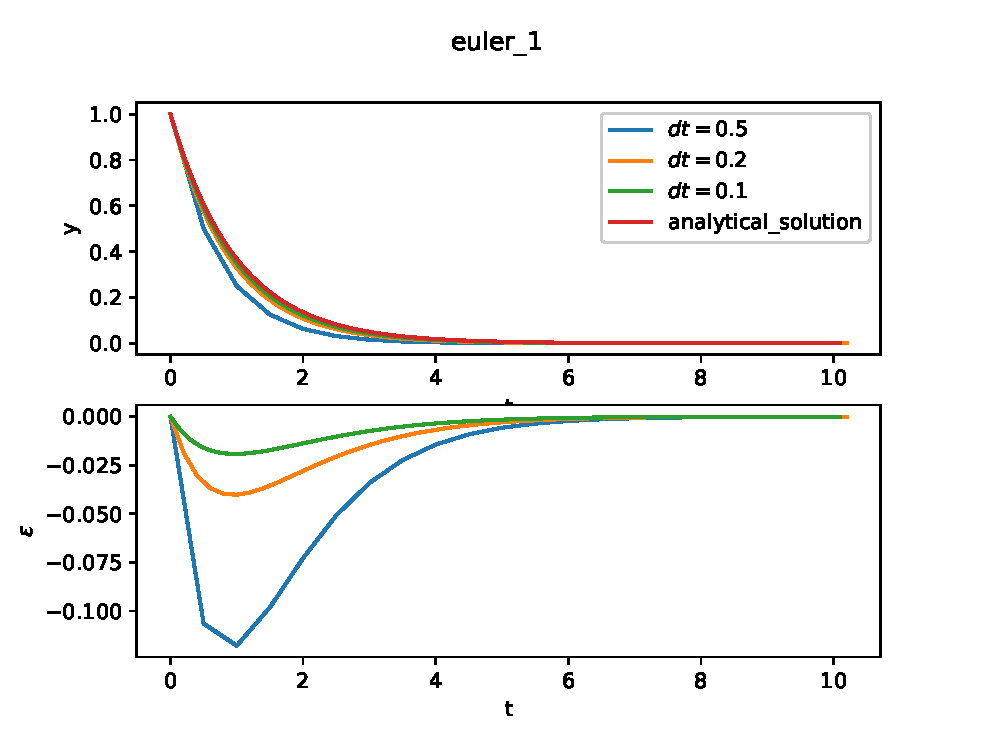
\epsfig{file=relaxation_euler_1.eps,width=\linewidth}
        \end{subfigure}
        \begin{subfigure}{0.49\linewidth}
            \centering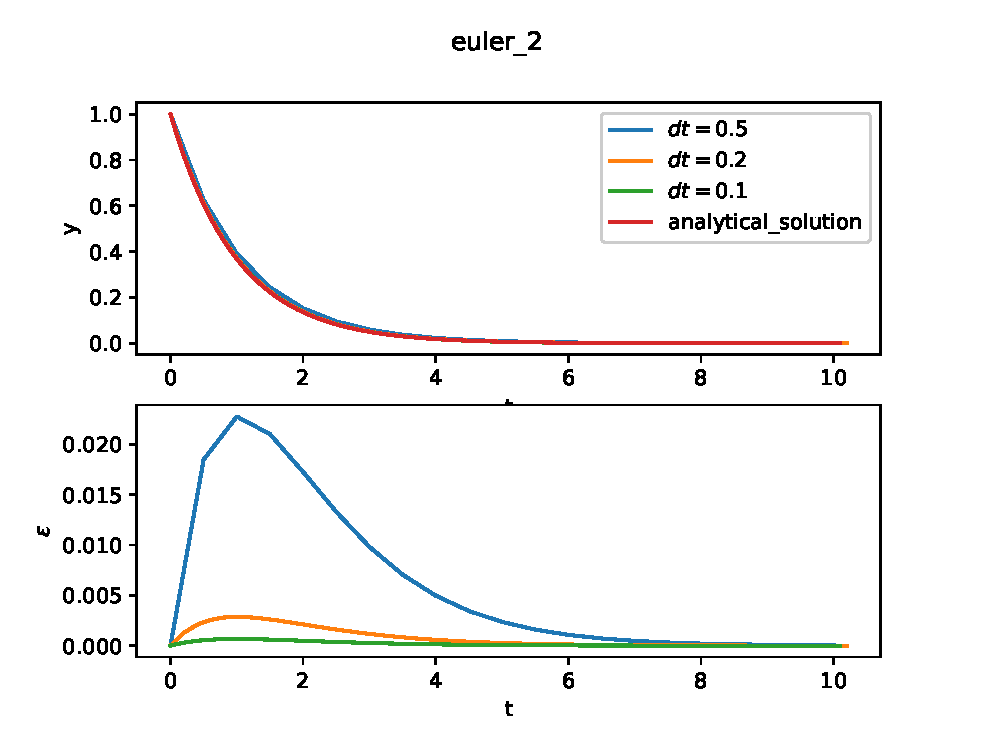
\epsfig{file=relaxation_euler_2.eps,width=\linewidth}
        \end{subfigure}
        \hfill
        \begin{subfigure}{0.49\linewidth}
            \centering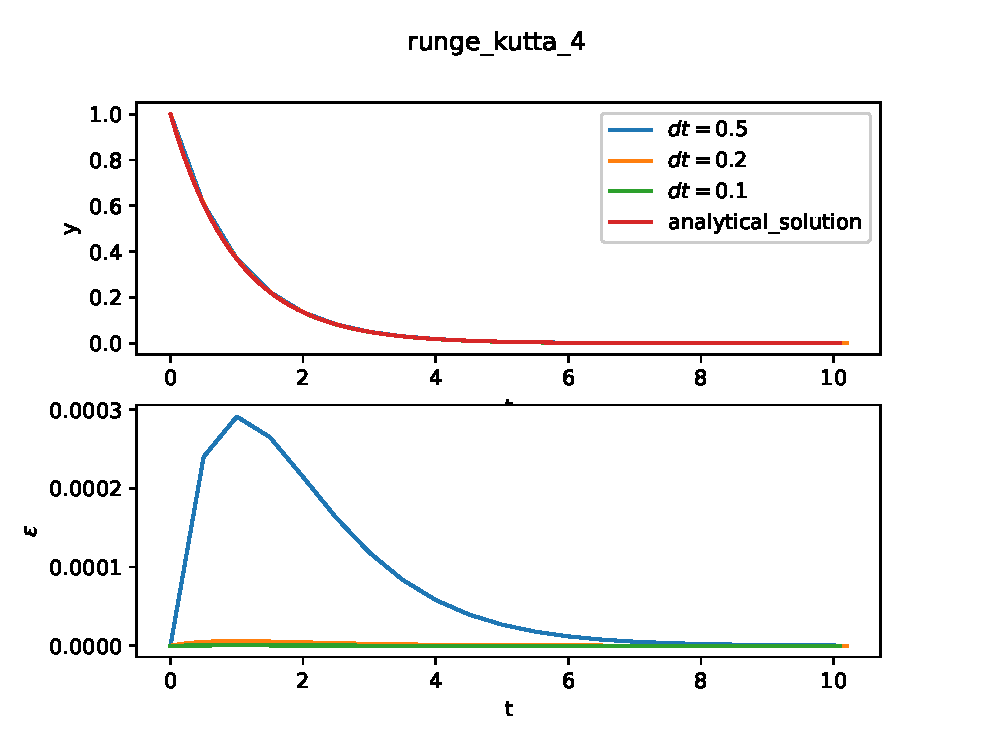
\epsfig{file=relaxation_runge_kutta_4.eps,width=\linewidth}
        \end{subfigure}
        \caption{
            \protect\small
            Integrace relaxační diferenciální rovnice ~\eqref{eq:relaxace} různými metodami a s různými časovými kroky.
        }	
        \label{fig:relaxace}
    \end{figure}

    \begin{itemize}
    \item \ghfile{python/ode/}{ode.py}: 
        Modul napsaný maximálně obecně, aby ho bylo možné použít na řešení libovolné diferenciální rovnice, a také soustav diferenciálních rovnic probíraných v sekci~\ref{sec:ODRn}.
        
        \begin{itemize}
        \item \code{euler_1}: 
            Integrační krok Eulerovy metody 1. řádu.
        \item \code{euler_2}: 
            Integrační krok Eulerovy metody 2. řádu.
        \item \code{runge_kutta_4}: 
            Integrační krok Runge-Kuttovy metody 4. řádu.
        \item \code{ode_solve}: 
            Integruje diferenciální rovnici danou pravou stranou prvního parametru \code{model} s počáteční podmínkou předanou parametrem \code{initial_condition}. 
            Integrační metodu lze specifikovat parametrem \code{integrator}, což je vlastně funkce $\phi(y_{i}, t_{i})$ z rovnice~\eqref{eq:phi}. 
            Délku kroku udává parametr \code{dt}.
            Funkce vrací pole hodnot řešení rovnice (soustavy rovnic) v jednotlivých časech a pole časů.
        \item \code{scipy_ode_solve}: 
            Integruje diferenciální rovnici pomocí funkce \code{odeint} z knihovny \code{sci\-py.integrate}. 
            Pozor, parametr \code{dt} zde neznačí integrační krok, nýbrž časový krok výsledného pole.
            Funkce \code{odeint} používá sofistikovaný řešitel diferenciálních rovnic s proměnným krokem.
            Pro podrobnosti můžete mrknout na \href{https://docs.scipy.org/doc/scipy/reference/generated/scipy.integrate.odeint.html}{dokumentaci} k této funkci.
    \end{itemize}

    \item \ghfile{python/ode/}{graphs.py}: 
        Vykresluje grafy srovnávající různé metody nebo různé kroky výpočtu.
        \begin{itemize}
        \item \code{plot_solution_error}:
            Vykreslí graf řešení diferenciální rovnice.
            Parametr \code{analyti\-cal_solution} je odkaz na přesné řešení dané diferenciální rovnice. 
            Je-li zadán, vykreslí se do grafu dva panely: jeden s hodnotami numerického řešení, druhý s rozdílem řešení numerického a přesného $\epsilon$ (akumulovaná diskretizační chyba dle  rovnice~\eqref{eq:AkumulovanaChyba}).
        \item \code{plot_compare_methods}:
            Vykreslí do jednoho obrázku řešení zadané diferenciální rovnice různými metodami.
            Z důvodu efektivnějšího kódu se v této funkci používá trochu složitější práce s panely, než jak je uvedeno ve vzorovém souboru \ghfile{python/basics/}{plot.py}.
        \item \code{plot_compare_steps}:
            Vykreslí do jednoho obrázku řešení zadané diferenciální rovnice s různými integračními kroky.
        \item \code{plot_cummulative_errors}:
            Řešení úlohy~\ref{task:KumulovanaChyba}.
        \end{itemize}

    \item \file{relaxation.py}:
        Soubor, který využívá integračních funkcí z modulu \ghfile{python/ode/}{ode.py} a vykreslovacích funkcí z modulu \ghfile{python/ode/}{graphs.py}
        pro řešení diferenciální rovnice pro relaxaci.
        \begin{itemize}
        \item Vyřeší diferenciální rovnici různými metodami, řešení nakreslí do jednoho grafu a porovná s teoretickou funkcí.
        \item Vyřeší diferenciální rovnici s různým časovým krokemm, řešení nakreslí do jednoho grafu a porovná s teoretickou funkcí.
        \item Nakreslí graf k úloze~\ref{task:KumulovanaChyba}.
        \end{itemize}
    \end{itemize}

    Příslušné grafy jsou zobrazeny na obrázku~\ref{fig:relaxace}.
    Je vidět, že chyba opravdu klesá s řádem metody a že čím je metoda vyššího řádu, tím rychleji chyba klesá se zmenšujícím se krokem.
\end{solution}

\begin{task}
\label{task:KumulovanaChyba}
    Rozšiřte kód tak, aby počítal průměrnou kumulovanou chybu
    \begin{equation}\label{eq:KumulovanaChyba}
        \mathcal{E}=\sqrt{\frac{1}{n}\sum_{i=0}^{n-1}\left(y_{i}-y(t_{i})\right)^{2}},
    \end{equation}
    kde $y(t)$ je analytické řešení diferenciální rovnice.
    Nakreslete závislost $\mathcal{E}(\Delta t)$ pro $\Delta t\in\langle0.002;0.1\rangle$ a pro různé metody.
    Jelikož očekáváme mocninnou závislost dle~\eqref{eq:RadMetodyODR}, kde exponent je tím větší, čím větší je řád metody, je výhodné graf $\mathcal{E}(\Delta t)$ kreslit v log-log měřítku.
    V Pythonu použijete místo \textnormal{\texttt{plot(...)}} funkci \textnormal{\texttt{loglog(...)}} z knihovny \textnormal{\texttt{matplotlib.pyplot}}.
    Ověřte, že získané křivky jsou v souladu s řády použitých metod.
\end{task}

\begin{solution}
    \begin{figure}[!htb]
        \centering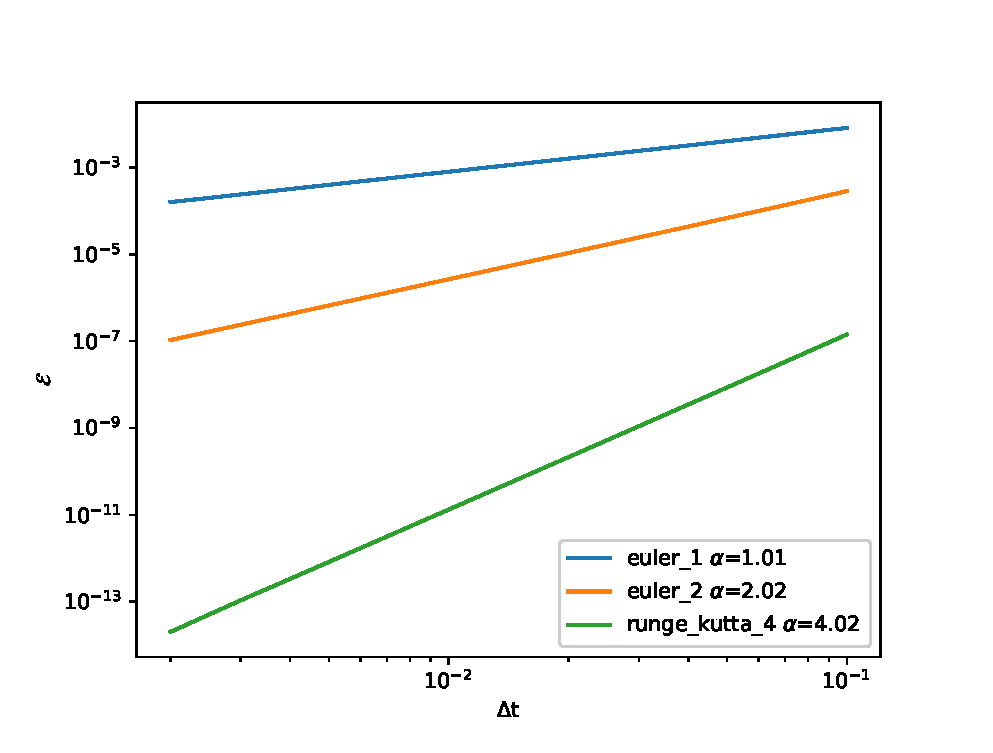
\epsfig{file=relaxation_cummulative_error.eps,width=0.7\linewidth}
        \caption{
            \protect\small
            Závislost průměrné kumulované chyby~\eqref{eq:KumulovanaChyba} na délce kroku $\Delta t$ vypočítaná a vykreslená pomocí funkce pro relaxační diferenciální rovnici.
        }
        \label{fig:relaxace_chyba}
    \end{figure}

    Řešení této úlohy vykreslí funkce \code{plot_cummulative_error} z modulu \ghfile{python/ode/}{graphs.py}. Graf je zobrazen na obrázku~\ref{fig:relaxace_chyba}.
    Body log-log grafu byla proložena přímka pomocí funkce lineární regrese \code{linregress} z knihovny \file{scipy.stats}.
    Nafitovaná směrnice $\alpha$ je uvedena v obrázku.
\end{solution}


\begin{task}
    Pomocí naprogramovaných metod vyřešte nelineární diferenciální rovnici
    \begin{equation}
        \label{eq:sinyt}
        \derivative{y}{t}=\sin\left(t y\right)
    \end{equation}
    s počáteční podmínkou $y_{0}=1$, $t_{0}=0$ a vykreslete graf jejího řešení.
\end{task}

\begin{solution}
    \begin{figure}[!htb]
        \centering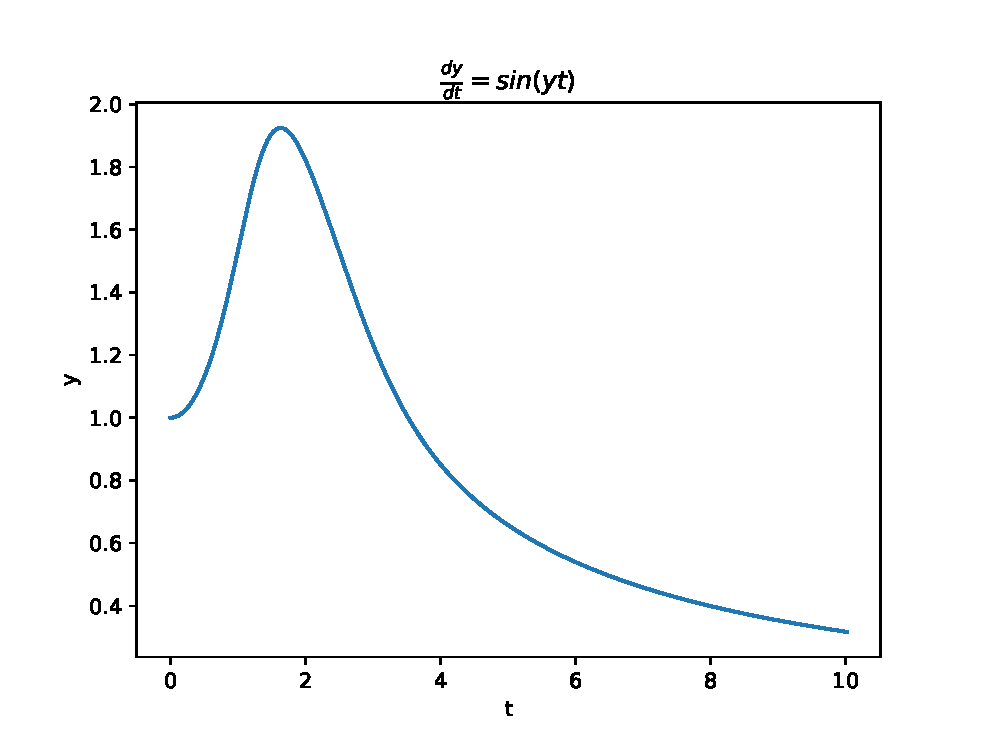
\epsfig{file=sinyt.eps,width=0.7\linewidth}
        \caption{
            \protect\small
            Řešení diferenciální rovnice~\eqref{eq:sinyt} s počáteční podmínkou $y(0)=1$.
            Použitá metoda: Runge-Kutta, časový krok $\Delta t=0.02$.
        }
        \label{fig:sinyt}
    \end{figure}

    Řešení je v souboru \ghfile{python/ode/}{sinyt.py}.
    Graf vypočítané funkce je na obrázku~\ref{fig:sinyt}.
\end{solution}


\section{Soustavy diferenciálních rovnic 1. řádu}
\label{sec:ODRn}
    Každou obyčejnou diferenciální rovnici $n$-tého řádu lineární v nejvyšší derivaci lze převést na~soustavu $n$ obyčejných diferenciálních rovnic prvního řádu ve tvaru
    \begin{equation}\label{eq:ODR}
        \derivative{\vector{y}}{t}=\vector{f}(\vector{y},t),
    \end{equation}
    kde $\vector{y}=\vector{y}(t)$ je vektor hledaných funkcí a $\vector{y}(t_{0})=\vector{y}_{0}$ vektor počáteční podmínky.

    \begin{example}
        Pohybovou rovnici
        \begin{equation}
            Ma=F(x),
        \end{equation}
        kde $M$ je hmotnost pohybujícího se tělesa, $x=x(t)$ jeho poloha a $a=a(t)=\d^{2}x/\d t^{2}$ zrychlení převedeme na~dvě diferenciální rovnice prvního řádu zavedením rychlosti $v=v(t)=\d x/\d t$:\footnote{
            Tato soustava rovnic odpovídá Hamiltonovým pohybovým rovnicím, se kterými se seznámíte v přednášce Teoretická mechanika.
        }
        \begin{equation}
            \derivative{}{t}\makematrix{x \\ v}=\makematrix{v \\ \frac{1}{M}F(x)},
        \end{equation}
        tj. vektor funkce pravých stran podle rovnice~\eqref{eq:ODR} je
        \begin{equation}
            \vector{f}(\vector{y},t)=\makematrix{v \\ \frac{1}{M}F(x)}
        \end{equation}
        kde $\vector{y}\equiv\makematrix{x \\ v}$.
    \end{example}

    \begin{example}
    Pohybová rovnice pro harmonický oscilátor (matematické kyvadlo s malou výchylkou) při volbě jednotek $M=\Omega=1$, kde $M$ je hmotnost kmitající částice a $\Omega$ její rychlost, zní
    \begin{align}
        a&=\derivative[2]{x}{t}=-x &&\Longleftrightarrow &
        \derivative{}{t}\makematrix{x \\ v}&=\makematrix{v \\ -x}
    \end{align}

    \end{example}

    \begin{voluntary}
    Převeďte na soustavu obyčejných diferenciálních rovnic prvního řádu rovnici třetího řádu pro Hiemenzův tok
    \begin{equation}
        x'''+xx''-x'^{2}+1=0.
    \end{equation}
    \end{voluntary}

    \begin{solution}
    Hledaná soustava diferenciálních rovnic je
    \begin{equation}
        \derivative{}{t}\makematrix{x \\ v \\ a}=\makematrix{v \\ a \\ -xa+v^{2}-1}.
    \end{equation}
    \end{solution}

    Drtivá většina knihoven a algoritmů pro integraci obyčejných diferenciálních rovnic počítá s rovnicemi ve~tvaru~\eqref{eq:ODR}.

\subsection{Symplektické algoritmy}
    Jedná se o speciální algoritmy navržené pro řešení pohybových differenciálních rovnic.
    Od běžných algoritmů je odlišuje to, že zachovávají objem fázového prostoru, a~tedy i energii (zatímco u obecných algoritmů se energie s integračním časem mění a většinou roste).
    
    V praxi se ze~symplektických algoritmů používá nejčastěji \emph{Verletův algoritmus}.
    Pro diferenciální rovnici 2. řádu ve tvaru 
    \begin{equation}\label{eq:EM}
        M\derivative[2]{x}{t}=F(x),
    \end{equation}
    což je pohybová rovnice pro jeden hmotný bod o hmotnosti $M$, na který působí časově neproměnná síla $F(x)$, má Verletův algoritmus tvar
    \begin{align}
        x_{i+1}&=x_{i}+v_{i}\Delta t+\frac{1}{2}a_{i}\Delta t^{2},\nonumber\\
        v_{i+1}&=v_{i}+\frac{1}{2}\left(a_{i+1}+a_{i}\right)\Delta t,
        \label{eq:Verlet}
    \end{align}
    kde $a_{i}\equiv F(x_{i})/M$ je zrychlení částice.

    Verletův algoritmus se používá nejčastěji v molekulární dynamice k simulaci pohybu velkého množství vzájemně interagujících částic.
    Jedná se o velmi rychlou a efektivní metodu.

    Řád Verletova algoritmu je $p=2$. 
    Symplektické algoritmy s vyšším řádem existují, avšak v praxi se nepoužívají.

\newpage
{\color{red}\subsection{Domácí úkol na 30.3.2021}}
\begin{task}
    Rozšiřte kód naprogramovaný v úkolu~\ref{task:ODR1} tak, aby fungoval pro libovolně velkou soustavu obyčejných diferenciálních rovnic.
    Využijte k tomu funkce pro práci s řadami z knihovny \file{numpy} popsané v sekci~\ref{sec:numpy}.
    Vyřešte diferenciální rovnici harmonického oscilátoru 
    \begin{equation}\label{eq:HO}
        \derivative[2]{x}{t}=-x
    \end{equation}
    s počátečními podmínkami $x_{0}=0$, $x'_{0}\equiv v_{0}=1$, $t_{0}=0$ a porovnejte řešení různými metodami s analytickým řešením $x(t)=\sin t$.
    Jako časový krok volte například $\Delta t=0.1$ a $\Delta t=0.01$ a počítejte na časovém intervalu $t\in\langle 0;30\rangle$.
\end{task}    

\begin{solution}
\label{sol:ODRn}
    Metody jsou naprogramovány v souborech \ghfile{python/ode/}{ode.py} (integrační metoda), \ghfile{python/ode/}{graphs.py} (vykreslování grafů) a jsou podrobně diskutování v řešení úlohy~\ref{sol:ODR1}.
    Soubor \ghfile{python/ode/}{ho.py} obsahuje pravé strany diferenciálních rovnic harmonického oscilátoru (funkce \code{ho}) a volá všechny výpočetní a vykreslovací funkce.
    Navíc obsahuje následující funkce:
    \begin{itemize}
    \item \code{ho_solution}:
        Přesné řešení pohybové rovnice harmonického oscilátoru s počáteční podmínkou $x_{0}=0,x'_{0}=1,t_{0}=0$, jímž je funkce $x(t)=\sin t$.
    \item \code{ho_energy}:
        Pro vstupní polohu a rychlost (nebo pole poloh a rychlostí) vrátí energii harmonického oscilátoru.
    \end{itemize}

    \begin{figure}[!htb]
        \begin{subfigure}{0.49\linewidth}
            \centering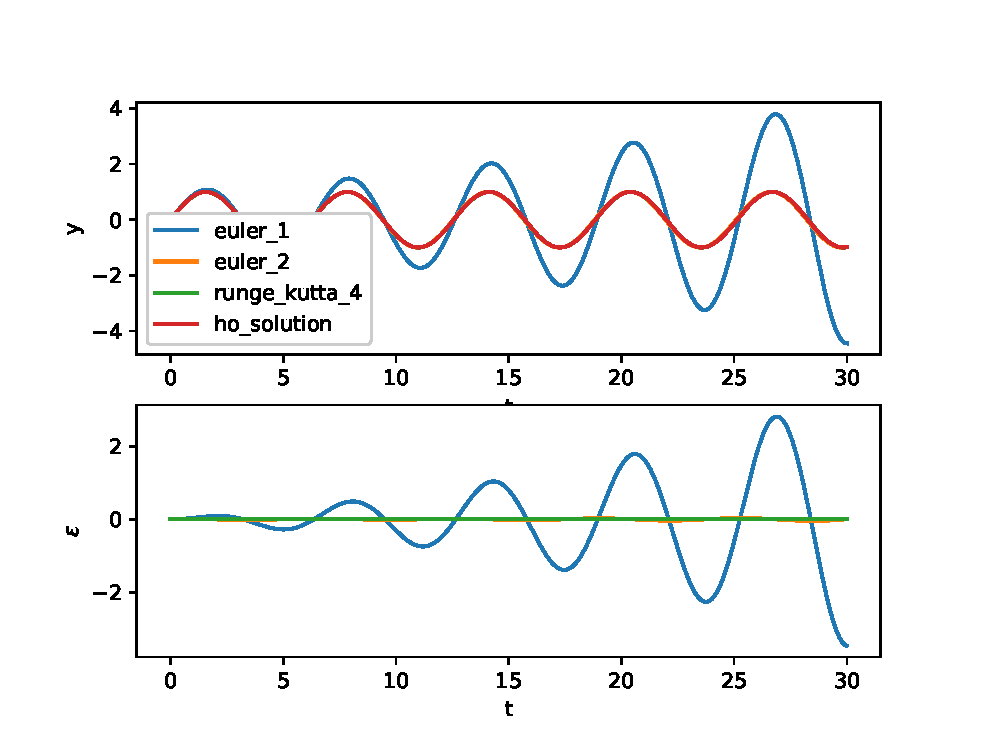
\epsfig{file=ho_methods.eps,width=\linewidth}
        \end{subfigure}
        \hfill
        \begin{subfigure}{0.49\linewidth}
            \centering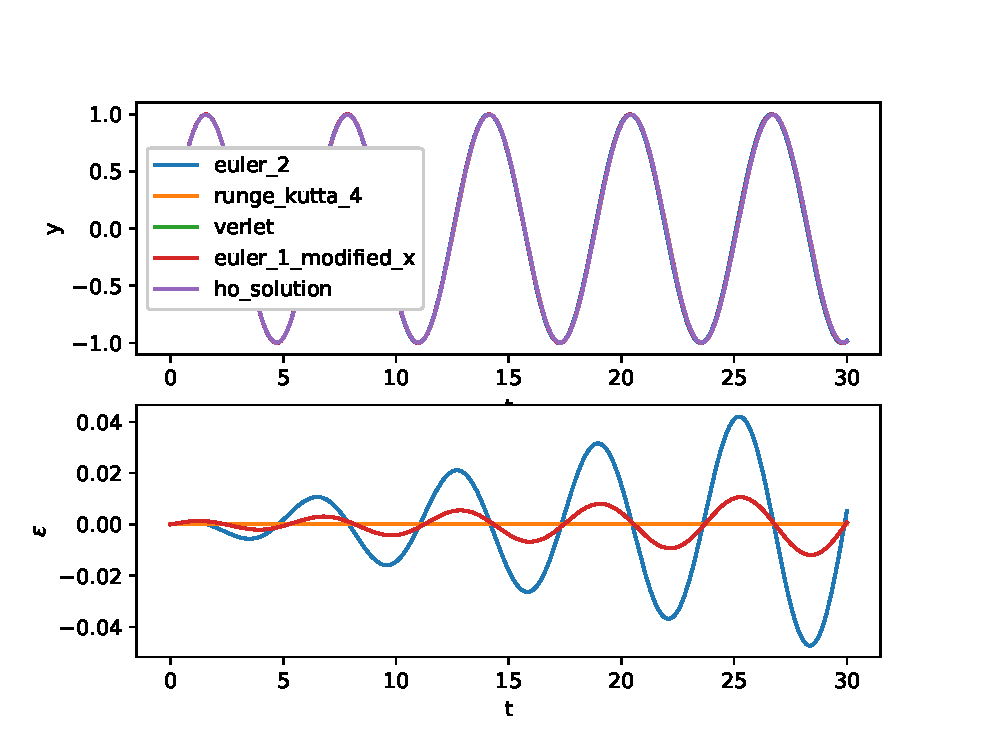
\epsfig{file=ho_symplectic.eps,width=\linewidth}
        \end{subfigure}
        \begin{subfigure}{0.49\linewidth}
            \centering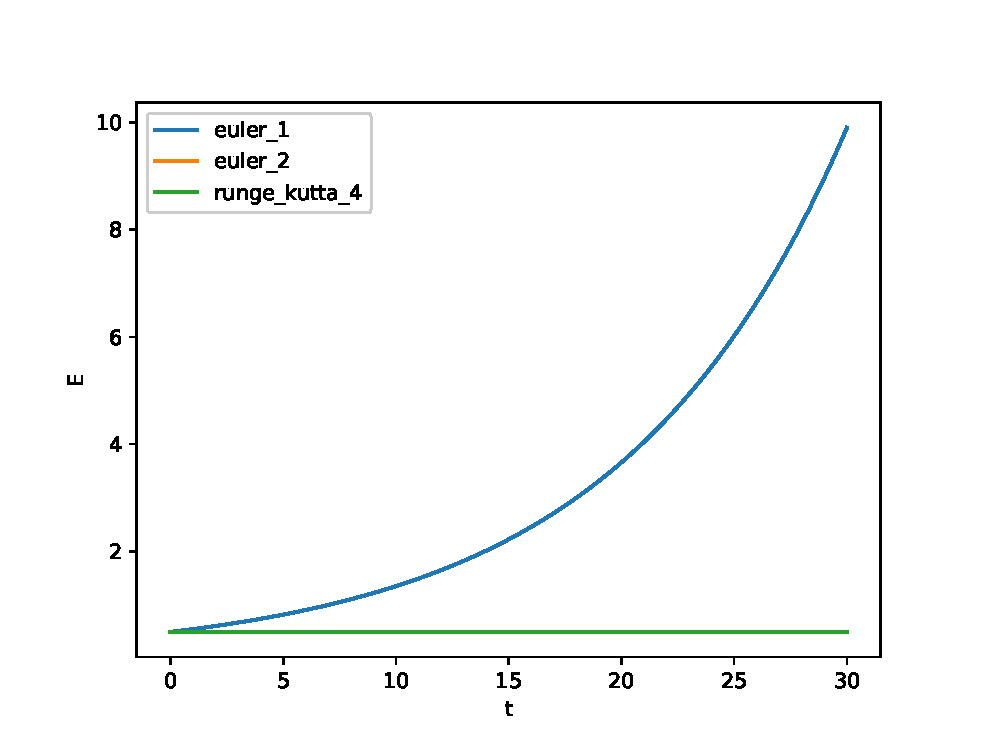
\epsfig{file=ho_energy.eps,width=\linewidth}
        \end{subfigure}
        \hfill
        \begin{subfigure}{0.49\linewidth}
            \centering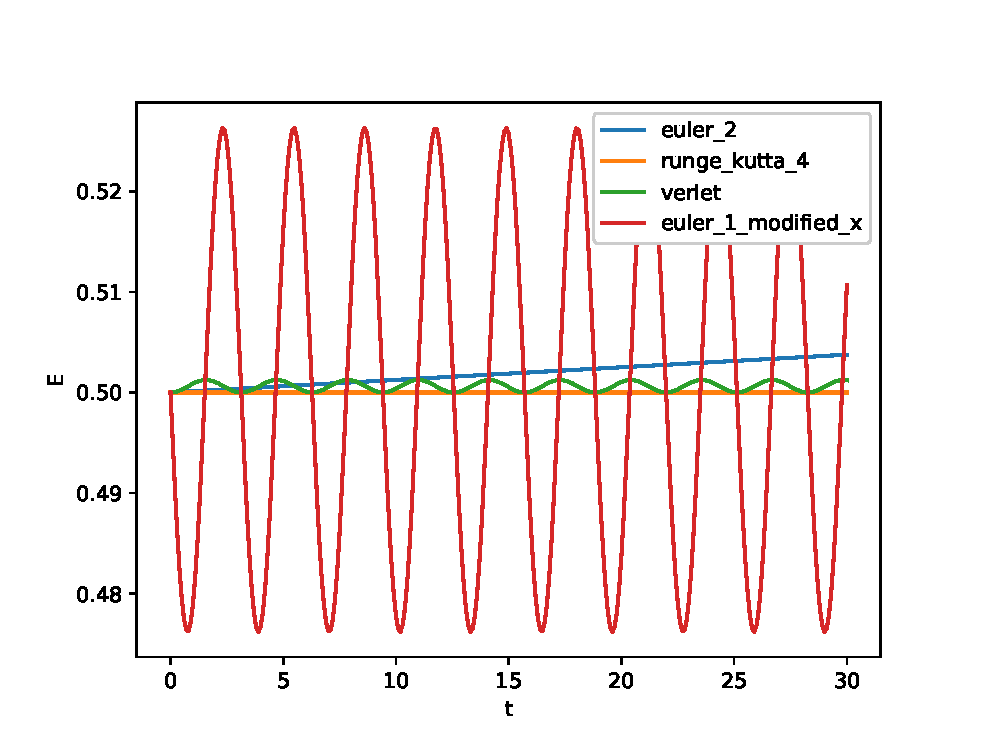
\epsfig{file=ho_energy_symplectic.eps,width=\linewidth}
        \end{subfigure}
        \caption{
            \protect\small
            Integrace diferenciální rovnice harmonického oscilátoru~\eqref{eq:HO} různými metodami.
            Časový krok je $\Delta t=0.1$.
            \emph{Levý sloupec:} všechny metody.
            \emph{Pravý sloupec:} Bez eulerovy metody 1. řádu a včetně symplektických metod.
            \emph{1.~řádek:} hodnoty $y(t)$.
            \emph{2.~řádek:} Akumulované diskretizační chyby dle~\eqref{eq:AkumulovanaChyba}.
            Pro Eulerovu metodu 1. řádu je obalová křivka divergence numerického od analytického řešení očividně exponenciální v čase.
            \emph{3.~řádek:} energie~\eqref{eq:HOE}. 
            Pro Eulerovy metody energie roste.
            Energie se mění i pro Runge-Kuttovu metodu (pro tento systém energie s časem klesá), avšak změna je řádově menší než pro ostatní metody, a tudíž není na grafech při daném měřítku svislé osy vidět.
            Naopak pro Verletův algoritmus a pro \uv{předbíhající} Eulerovu metodu energie osciluje okolo počáteční energie $E=\frac{1}{2}$.
        }	
        \label{fig:HO}
    \end{figure}

    Příslušné grafy jsou zobrazeny na obrázku~\ref{fig:HO}.
\end{solution}


\begin{task}
    Naprogramujte Verletův algoritmus~\eqref{eq:Verlet}.
    Ukažte, že zatímco při použití Eulerovy metody nebo Runge-Kuttovy metody energie systému v průběhu výpočtu roste, Verletův algoritmus energii zachovává.
    Energie bezrozměrného harmonického oscilátoru~\eqref{eq:HO} je dána vzorcem
    \begin{equation}\label{eq:HOE}
        E=\frac{1}{2}\left(x^{2}+v^{2}\right).
    \end{equation}
\end{task}

\begin{solution}
    Symplektický Verletův algoritmus je naprogramován v souboru \ghfile{python/ode/}{symplectic.py}.
    Toto vzorové řešení bude fungovat \emph{jen} pro jednu pohybovou rovnici, tj. pro jednu diferencální rovnici původně druhého řádu přepsanou na dvě diferenciální rovnice prvního řádu, přičemž první rovnice musí být pro souřadnici, druhá pro rychlost. 
    Řešení lze samozřejmě rozšířit na více pohybových rovnic.

    V souboru \ghfile{python/ode/}{symplectic.py} je i funkce \code{plot_energy}, která vykreslí graf závislosti $E(t)$.
    Energie je znázorněna v panelech na třetím řádku na obrázku~\ref{fig:HO}.
    Harmonický oscilátor je konzervativní systém (zachovává energii), pozorovaná rostoucí energie je způsobena nepřesností integračních metod.
    U symplektických algoritmů energie slabě osciluje okolo střední hodnoty, která však i pro velmi dlouhé časy zůstává na přesné hodnotě $E=\frac{1}{2}$.
\end{solution}


\begin{task}
    Eulerovu metodu 1. řádu lze pro soustavy dvou diferenciálních rovnic 1. řádu vylepšit následující záměnou:
    \begin{align}
        &\begin{matrix}
            x_{i+1}=x_{i}+v_{i}\Delta t \\
            v_{i+1}=v_{i}-x_{i}\Delta t 
        \end{matrix}
        &&\longrightarrow
        &\begin{matrix}
            x_{i+1}=x_{i}+v_{i}\Delta t \\
            v_{i+1}=v_{i}-x_{i+1}\Delta t 
        \end{matrix}
    \end{align}
    (vypočítáme $x_{i+1}$ a tuto hodnotu použijeme namísto hodnoty $x_{i}$ pro výpočet rychlosti $v_{i+1}$).
    Naprogramujte tuto metodu a pomocí výsledků úlohy~\ref{task:KumulovanaChyba} ukažte, že pro harmonický oscilátor se jedná o metodu 2. řádu.
\end{task}

\begin{solution}
    \uv{Vylepšené} Eulerovy metody jsou naprogramovány v souboru \ghfile{python/ode/}{symplectic.py}.
    Metoda s předbíhající se souřadnicí je označena \code{euler_1_modified_x}, metoda s předbíhající rychlostí pak \code{euler_1_modified_v}.
    Obě metody dávají velmi podobné výsledky, v grafech je proto uvedena jen první z nich.

    Řešení diferenciální rovnice harmonického osciátoru je znázorněno v pravém sloupci obrázku~\ref{fig:HO}.
    Je vidět, že so se přesnosti týče, vylepšená Eulerova metoda je srovnatelná s Verletovou metodou.
    Energie však osciluje trochu víc.

    \begin{figure}[!htbp]
        \centering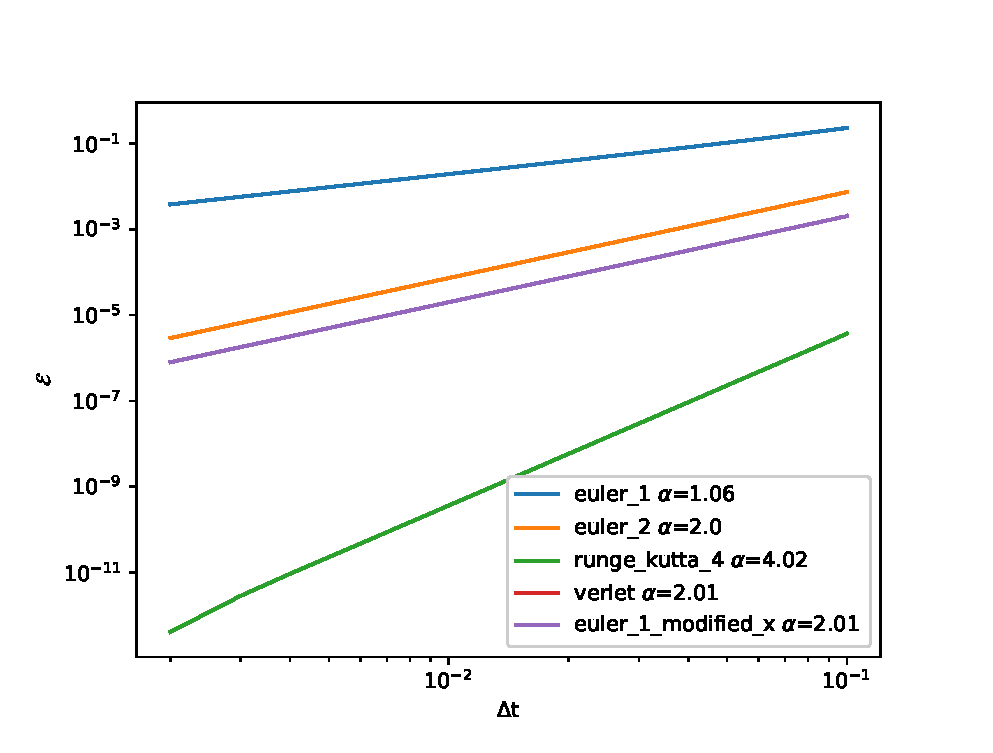
\epsfig{file=ho_cummulative_error.eps,width=0.7\linewidth}
        \caption{
            \protect\small
            Závislost průměrné kumulované chyby~\eqref{eq:KumulovanaChyba} na délce kroku $\Delta t$ vypočítaná a vykreslená pro soustavu diferenciálních rovnic pro harmonický osciátor.
            Zobrazeny jsou i symplektické metody.
        }
        \label{fig:ho_chyba}
    \end{figure}
    
    Řád metody lze určit na základě obrázku~\ref{fig:ho_chyba}.
    Jak u Verletovy metody, tak u vylepšené Eulerovy metody klesá průměrná kumulovaná chyba s druhou mocninou délky časového kroku $\delta t$, jedná se tedy o metody 2. řádu.
\end{solution}


\begin{task}
    Pohrajte si s řešením rovnice pro klesající exponenciálu
    \begin{equation}\label{eq:Exp2}
        \derivative[2]{x}{t}=x
    \end{equation}
    s počátečními podmínkami $x_{0}=1$, $x'_{0}=-1$.
    Přesvědčte se, že Verletova metoda a vylepšená Eulerova metoda z předchozího úkolu jsou nestabilní --- pro tuto rovnici v relativně krátkém čase začnou řešení exponenciálně divergovat.
\end{task}

\begin{solution}
    Řešení rovnice~\eqref{eq:Exp2} je v souboru \ghfile{python/ode/}{exp.py}.
    Soustava rovnic je analogická k soustavě harmonického oscilátoru --- liší se pouze znaménkem.
    Systém popsaný touto rovnicí \emph{není konzervativní} --- nelze nadefinovat zachovávající se veličinu, která by měla význam energie.

    \begin{figure}[!htbp]
        \centering
        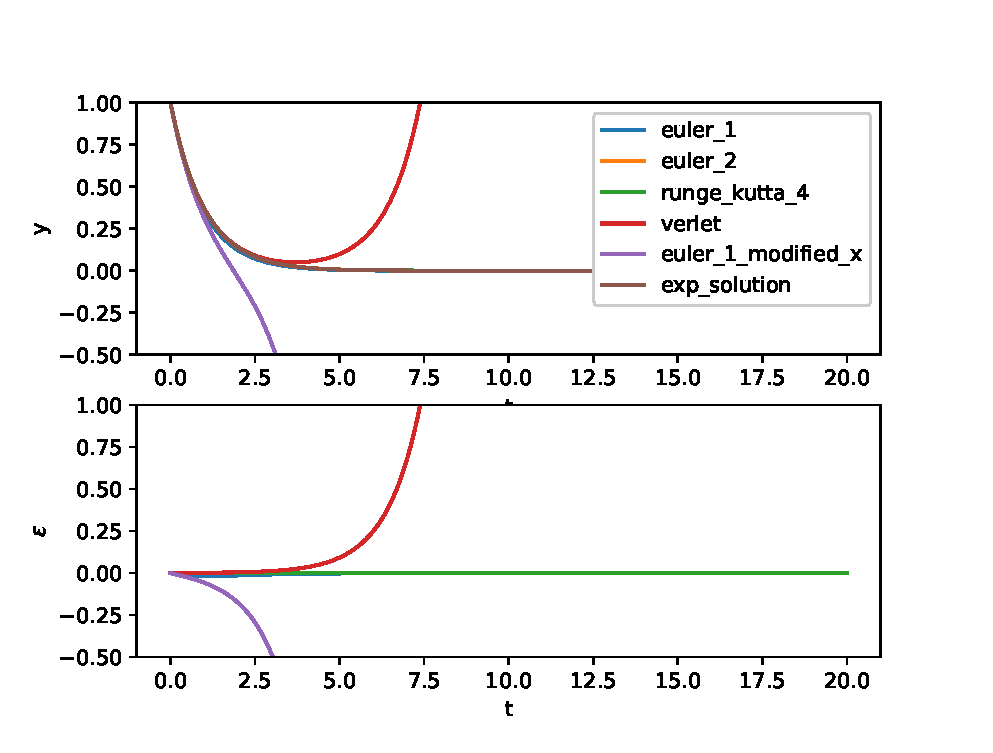
\epsfig{file=exp_divergence.eps,width=0.8\linewidth,keepaspectratio}
        \caption{
            \protect\small
            Totéž jako v obrázku~\ref{fig:HO}, avšak pro exponenciálně klesající systém daný rovnicí~\eqref{eq:Exp2}.
            Symplektické algoritmy jsou nestabilní.
            }	
        \label{fig:Exp2}
    \end{figure}
    
    Z obrázku~\ref{fig:Exp2} je vidět, že symplektické algoritmy jsou nestabilní, a tudíž nejsou na tento typ úlohy vhodné, což je pochopitelné, protože jsou navrženy pouze pro energii zachovávající systémy.
    Příčinu nestability lze nahlédnout i z obecného řešení rovnice~\eqref{eq:Exp2},
    \begin{equation}
        y(t)=A\e^{t}+B\e^{-t},
    \end{equation}
    přičemž my speciálními počátečními podmínkami vybíráme pouze exponenciálně klesající řešení.
    Symplektické algoritmy však v určitou chvíli \uv{překmitnou} na exponenciálně rostoucí řešení, což způsobí pozorovanou divergovat.
\end{solution}

\begin{task}
    Vyřešte nelineární soustavu tří diferenciálních rovnic pro jednoduchý Lorenzův model vedení tepla v atmosféře
    \begin{align}
        \derivative{x}{t}&=\sigma(y-x),\nonumber\\
        \label{eq:Lorenz}
        \derivative{y}{t}&=x(\rho-z)-y,\\
        \derivative{z}{t}&=xy-\beta z\nonumber
    \end{align}
    s hodnotami parametrů $\sigma=10$, $\rho=28$ a $\beta=8/3$, počátečními podmínkami $(x_0, y_0, z_0)=(1,1,1)$ (na počátečních podmínkách zase tolik nezáleží), s krokem $\Delta t=0.01$ a na časovém intervalu $t\in\langle0,100\rangle$.
    Vykreslete graf $z(x)$.
    Výsledná křivka je slavný Lorenzův podivný atraktor ve tvaru motýlích křídel, krerý zpopularizoval teorii klasického chaosu.
\end{task}

\begin{solution}
    Řešení Lorenzova systému diferenciálních rovnic je jednoduchou aplikací kódu naprogramovaného v úloze~\ref{sol:ODRn} a lze ho nalézt v souboru \ghfile{python/ode/}{lorenz.py}.
    Příslušnou projekci trojrozměrné trajektorie do 2D roviny $(x,z)$ lze nalézt na obrázku~\ref{fig:Lorenz}.

    \begin{figure}[!htbp]
        \centering
        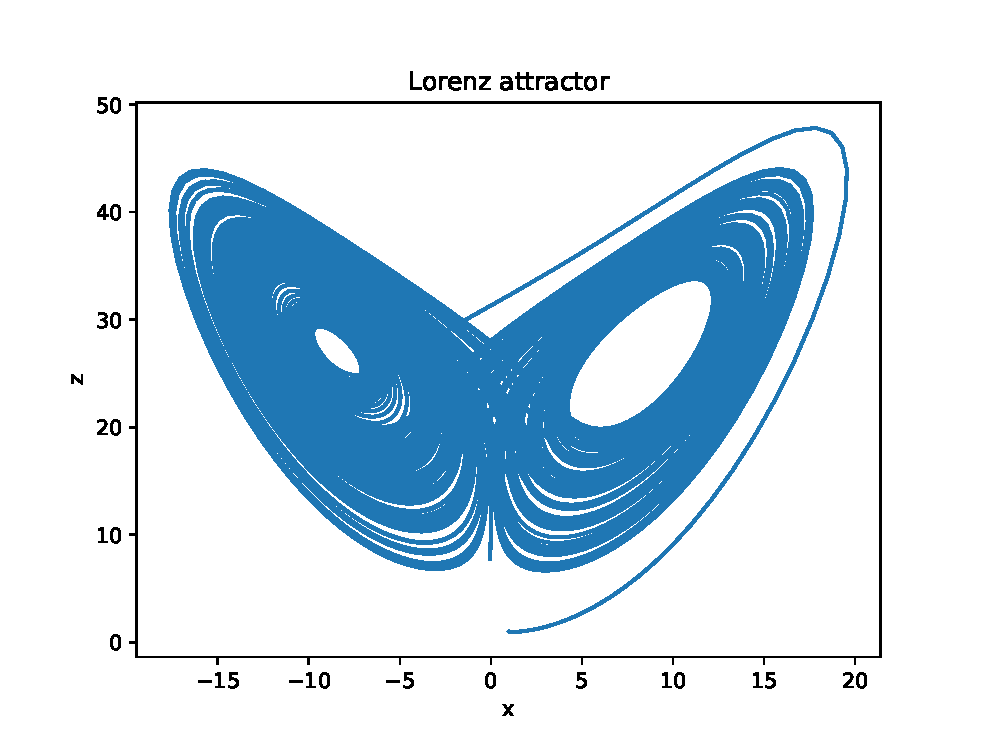
\epsfig{file=lorenz.eps,width=0.7\linewidth,keepaspectratio}
        \caption{
            \protect\small
                Lorenzův systém~\eqref{eq:Lorenz} integrovaný pomocí Runge-Kuttovy metody 4. řádu na časovém intervalu $t\in\langle0;100\rangle$ s krokem $\Delta t=0.01$.
            }	
        \label{fig:Lorenz}
    \end{figure}
\end{solution}

\subsection{Shrnutí}
\begin{itemize}
\item 
    Řešitelé obyčejných diferenciálních rovnic převážně pracují se soustavami diferenciálních rovnic prvního řádu.
    Na tento tvar není obtížné diferenciální rovnici vyššího řádu převést.

\item
    Nejčastěji se používají jednokrokové metody, jejichž hlavní výhoda je v možnosti jednoduše dle potřeby měnit délku kroku (metody s adaptivním krokem).

\item 
    Přesnost řešení závisí na řádu metody $p$ a na délce integračního kroku $\Delta t$.
    Čím je řád metody vyšší, tím rychleji klesá chyba se zmenšujícícm se krokem.
    V praxi, pokud nechcete svěřit svůj probém černé skříňce ve formě nějaké hotové knihovny, se velmi často používá Runge-Kuttova metoda 4. řádu, která je jednoduchá na implementaci, je stabilní a rychlá.

\item
    Symplektické metody, z nichž nejběžnější je Verletova metoda, jsou výhodné k modelování fyzikálních systémů zachovávajících energii.
    Pro nekonzervativní systémy nejsou vhodné. 
\end{itemize}
A hlavně, nyní již umíte jen pomocí sčítání a násobení vypočítat a nakreslit průběh goniometrické funkce sinus.


\section{Náhodná procházka}\label{sec:NahodnaProchazka}
    Náhodná procházka je jeden ze základních prostředků, jak simulovat velké množství nejen fyzikálních procesů (například pohyb Brownovské částice, fluktuace akciového trhu, cestu opilce z~hospody atd.).
    V dalších cvičeních si ukážeme, jak se pomocí náhodné procházky dá jednoduše hledat minimum funkcí (a to i funkcí více proměnných). 

    Algoritmus pro náhodnou procházku je následující: v každém časovém kroku uděláme krok v~$d$-rozměrném prostoru $\vector{y}_{i}\rightarrow\vector{y}_{i+1}$ takovým způsobem, aby pravděpodobnost pohybu do všech směrů byla stejná.
    Délka kroku $s$ se volí buď náhodná, nebo konstantní.

    K simulování náhodných procesů slouží algoritmy generující pseudonáhodná čísla, což jsou čísla, která mají statistické vlastnosti blízké vlastnostem skutečných náhodných čísel, avšak jsou počítána jednoduchými deterministickými algoritmy.
    Náhodná čísla se generují od počáteční tzv. \emph{násady} (seed), kterou lze explicitně zadat, a tím posloupnost náhodných čísel přesně zreprodukovat (díky tomu, že generující algoritmy jsou deterministické).
    Pokud násada není explicitně zadána, knihovny pro generování pseudonáhodných čísel většinou volí systémový čas, takže při každém spuštění programu dostáváme posloupnost odlišnou.

    Základní funkce a postupy pro generování náhodných čísel v Pythonu jsou uvedeny v sekci~\ref{sec:PseudonahodnaCisla}.

    {\color{red}\subsection{Domácí úkol na 6.4.2021}}
    \begin{task}
        Naprogramujte náhodnou procházku ve 2D rovině.
        Délku kroku volte konstantní $s=1$, směr volte náhodně.
        Začněte z bodu $(x,y)=(0,0)$ a procházku ukončete poté, co opustíte oblast tvaru čtverce o hraně délky $2a$.
        Uchovávejte celou procházku v poli či seznamu.
        Nakonec trajektorii vykreslete do~grafu.
    \end{task}

    \begin{solution}
        Řešení je naprogramováno v souboru \ghfile{python/randomwalk/}{2d.py}.
        \begin{itemize}
            \item \code{random_direction_2d} vrátí náhodný směr ve 2D rovině [generuje náhodný úhel $\phi$, směr je dán jednotkovým vektorem se složkami $(\cos\phi,\sin\phi)$].
            \item \code{random_walk_2d} vykreslí do grafu náhodnou procházku s \code{num_steps} kroky omezenou ve čtverci rozměru $2*$\code{box_size}$\times2*$\code{box_size} a náhodnou procházku vrátí.
            \item \code{random_walk_2d_interactive} generuje náhodnou procházku a vykresluje ji do grafu krok po kroku.
                Musí být zapnutý interaktivní mód vykreslování \code{plt.ion()} a v prostředí Spyder vypnuto použítí inline grafů příkazem \code{\%matplotlib auto} v konzoli REPL.
                Tato funkce implementuje i cyklické okrajové podmínky.
        \end{itemize}
        Vzorový kód je napsán takovým způsobem, aby mohl být přímočaře rozšířen pro vícerozměrnou náhodnou procházku.
    \end{solution}
    
    \begin{task}
        Upravte náhodnou procházku tak, aby počítala s cyklickými okrajovými podmínkami.
        To znamená, že pokud opustíte oblast čtverce jednou jeho stranou, objevíte se na straně protilehlé (jako kdybyste okraje čtverce zavinuli a slepili).
        Výpočet ukončete poté, co uděláte $n$ kroků.
    \end{task}

    \begin{solution}
        Cyklické okrajové podmínky jsou naprogramovány ve funkci \code{random_walk_2d_inter\-active} v souboru \ghfile{python/randomwalk/}{2d.py}.
        Stejně je lze naprogramovat i do funkce \code{random_walk_2d}, výsledný graf však nebude vypadat příliš hezky.
    \end{solution}

    \begin{task}\label{task:NahodnaProchazka}
        Zamyslete se nad tím, jak byste realizovali náhodnou procházku s konstantní délkou kroku v $d>2$ rozměrech, a zkuste své řešení naprogramovat.
        Zásadní je dodržet požadavek, aby pohyb do jakéhokoliv směru nastával se stejnou pravděpodobností (esence úlohy tedy spočívá v generování náhodného směru v $d$-rozměrném prostoru).
    \end{task}

    \begin{solution}
        Zatímco pro směr ve 2D rovině stačí náhodě generovat jeden úhel (předchozí úloha), vícerozměrné úlohy jsou komplikovanější.
        Přímé rozšíření 2D případu do 3D (či do vyšších dimenzí) za generování více úhlů a použití (hyper-)sférických souřadnic k cíli nevede --- takto otrocky generované směry upřednostňují okolí pólů před rovníkem (rozmyslete).
        K úspěšnému generování náhodného kroku je nutné využít jeden z následujících algoritmů:
        \begin{enumerate}
            \item Hyperkoule vepsaná v hyperkrychli.
                \begin{enumerate}
                    \item Nagenerujeme bod v hyperkrychli o hraně délky $2$, tj. generujeme vektor $\vector{v}$ s $d$ složkami, přičemž každá složka je náhodné číslo z rovnoměrného rozdělení $(-1,1)$.
                    \item Zkontrolujeme, zda bod leží uvnitř vepsané jednotkové koule například tak, že spočítáme jeho normu $v=\abs{\vector{v}}$ a porovnáme, zda $n\leq1$.
                    \item Pokud ne, opakujeme postup od začátku.
                        Pokud ano, nagenerovaný bod promítneme na~jednotkovou kouli (jinými slovy vektor $\vector{v}$ nanormujeme) a získaný jednotkový vektor $\vector{\hat{v}}\equiv\vector{v}/v$ udává hledaný směr. 
                \end{enumerate}
                Tato metoda je nesmírně neefektivní, pokud je dimenze $d$ vysoká, poněvadž v tom případě většina nagenerovaných bodů leží vně vepsané hyperkoule a je zahozena.
                Poměr celkového počtu nagenerovaných bodů ku úspěšným zásahům vnitřku hyperkoule lze snadno spočítat.
                Objem hyperkrychle o hraně délky $2$ je
                \begin{equation}
                    V_{d}^{(\text{krychle})}=2^{d},
                \end{equation}
                objem vepsané hyperkoule o poloměru $1$ je
                \begin{equation}
                    V_{d}^{(\text{koule})}=\frac{\pi^{\frac{d}{2}}}{\Gamma\left(\frac{d}{2}+1\right)},
                \end{equation}
                kde $\Gamma$ je Eulerova gama funkce.
                Vzájemný poměr
                \begin{equation}
                    \eta_{d}\equiv\frac{V_{d}^{(\text{krychle})}}{V_{d}^{(\text{koule})}}=\left(\frac{2}{\sqrt{\pi}}\right)^{d}\Gamma\left(\frac{d}{2}+1\right)
                \end{equation}
                udává, kolik bodů musíme průměrně nagenerovat, abychom se trefili do hyperkoule (reciproká hodnota $1/\eta_{d}$ určuje pravděpodobnost, že se do hyperkoule trefíme).
                Zatímco pro $d=3$ je $\eta_{3}\approx1.91$, pro $d=10$ již $\eta_{10}\approx401$, tj. pro nalezení jednoho náhodného směru v desetirozměrném prostoru musíme nagenerovat v průměru přes $4000$ náhodných čísel.
                Z posledního vztahu je vidět, že s rostoucí dimenzí roste $\eta_{d}$ exponenciálně.

                Z tohoto výpočtu také vyplývá, že pokud bychom nezahazovali body ležící mimo hyperkouli, pak bychom ve výsledné procházce výrazně upřednosťnovali pohyb podél diagonál, a to tím více, čím vyšší je dimenzionalita procházky (u $d=10$ bychom podél diagonál vyrazili s více než $99\%$ pravděpodobností).
                
            \item Náhodný Gaussovský vektor.
                \begin{enumerate}
                    \item Nagenerujeme vektor $\vector{n}$ s $d$ složkami, přičemž každá složka je číslo z normálního Gaussovského rozdělení $N(0,1)$.
                    \item Vektor nanormujeme a získáme hledaný náhodný směr $\vector{\hat{n}}\equiv\vector{n}/n$. 
                \end{enumerate}
                Tato metoda je mnohem přímočařejší než předchozí, předpokladem je jen mít k dispozici generátor čísel vybraných z normálního rozdělení.

                Důkaz, že tato metoda dává opravdu náhodný směr v $d$ dimenzích, a další informace o metodě se nalézá v článcích~\cite{Muller1959,Marsaglia1972}.

            \item Speciální případ $d=3$ (náhodný let).
                \begin{enumerate}
                    \item Generujeme dvě náhodná čísla $\xi_{1,2}$ z rovnoměrného rozdělení na intervalu $\langle0;1)$.
                    \item Sférické úhly jednotkového směru jsou pak
                        \begin{align}
                            \phi&=2\pi\xi_{1},\nonumber\\
                            \theta&=\arccos\left(1-2\xi_{2}\right),
                        \end{align}
                        takže hledaný jednotkový vektor $\vector{\hat{n}}$ do náhodného směru má komponenty
                        \begin{align}
                            \hat{n}_{x}
                                &=\sin\theta\cos\phi
                                =\sqrt{1-\left(1-2\xi_{2}\right)^{2}}\cos2\pi\xi_{1},\nonumber\\
                            \hat{n}_{y}
                                &=\sin\theta\sin\phi
                                =\sqrt{1-\left(1-2\xi_{2}\right)^{2}}\sin2\pi\xi_{1},\\
                            \hat{n}_{z}
                                &=\cos\theta
                                =1-2\xi_{2}.\nonumber
                        \end{align}
                        Ve více rozměrech je tento přístup prakticky nerealizovatelný (vede na problém inverzních funkcí k funkcím daným řadou goniometrických funkcí).
                \end{enumerate}
            \end{enumerate}

            Náhodná procházka v $d$-rozměrném prostoru je naprogramována v souboru \ghfile{python/randomwalk/}{nd.py}.
            Funkce \code{ran\-dom_direction} generuje směr pomocí 1. metody, funkce \code{random_direction_gaussian} pomocí 2. metody.
            Spočítejte si náhodnou procházku pro $d=10$ oběma metodami.
            Uvidíte, že i~pro takto relativně \uv{malou} dimenzi je rozdíl ve výpočetních časech je dramatický.
    \end{solution}



\section{Hledání minima funkce}
    Náhodnou procházku lze úspěšně použít k hledání minima funkce obecně více proměnných.
    Představte si funkci dvou proměnných jako zvlněnou \uv{krajinu} v noci.
    Potřebujete se vrátit k chatě, která se nachází pod vámi hluboko v úkolí.
    Je tma a nevidíte jakým směrem se vydat.
    Zkusíte tedy udělat náhodný krok a pokud povede dolů, vykročíte.
    Pokud by však krok vedl nahoru, zůstanete na místě a zkusíte nový směr.

    Jednoduchá náhodná procházka funguje dobře pro funkce s jedním minimem.
    V obecném případě ale může mít funkce více lokálních minim a právě uvedený algoritmus skončí náhodně v jednom z nich, ze kterého se již nedokáže dostat ven.
    Přitom rozhodně nemusí jít o minimum nejhlubší (globální).
    
    Hledání globálního minima funkce mnoha proměnných je obecně velmi komplexní problém.
    Dva nejjednodušší postupy, kterými můžeme vylepšit stávající metodu pomocí náhodné procházky, jsou následující:
    \begin{itemize}
        \item Provedeme několik náhodných procházek, které obecně dojdou do různých lokálních minim.
            Následně porovnáme konečné funkční hodnoty a vybereme to minimum, které má hodnotu nejnižší.
        \item Provedeme jednu náhodnou procházku doplněnou o \emph{Metropolisův algoritmus}. 
    \end{itemize}

\subsection{Metropolisův algoritmus}
    Metropolisův algoritmus rozšiřuje náhodnou procházku o konečnou teplotu.
    Je inspirován termodynamickým Boltzmannových rozdělením energie: 
    máme tepelnou energii, díky které můžeme při náhodné procházce s určitou pravděpodobností udělat krok i \uv{do kopce}, avšak čím je kopec strmější, tím bude pravděpodobnost takovéhoto kroku menší.
    
    Předpokládejme, že jsme na vrstevnici s funkční hodnotou $f$ a nová funkční hodnota po provedení kroku náhodné procházky by byla $f_{\text{nová}}>f$.
    Při minimalizaci pomocí obyčejné náhodné procházky bychom tento krok neprovedli.
    V Metropolisově algoritmu krok provedeme s pravděpodobností
    \begin{equation}
        p=\e^{\frac{f-f_{\text{nová}}}{T}},
    \end{equation}
    kde $T$ je parametr, který má roli \uv{teploty}: pokud $T=0$, žádný tepelný pohyb neexistuje, krok do kopce nikdy neprovedeme a vracíme se tak k obyčejné minimalizaci.
    Pokud $T\rightarrow\infty$, uděláme krok do kopce s pravděpodobností $p=1$,
    což znamená, že tepelný pohyb zcela převládá, my se pohybujeme zcela náhodně a potenciál pod sebou vůbec necítíme.
    
    V praxi je největší umění zvolit správnou hodnotu teploty.
    Pokud zvolíme teplotu nízkou, skončíme v lokálním minimu a už se z něj nedostaneme, pokud naopak příliš vysokou, budeme chaoticky procházet krajinou naší funkce a žádné minimum nenajdeme.
    Dobrá volba je začít spíš s~vyšší teplotou a teplotu postupně snižovat.
    Jakmile se ocitneme zaseklí v nějakém minimu, můžeme teplotu zase trochu zvýšit a tím vyzkoušet, zda se nepřesuneme do nějakého minima hlubšího.

\subsection{Minimalizace pomocí knihovny SciPy}
    Python obsahuje funkci pro hledání minima \code{\href{https://docs.scipy.org/doc/scipy/reference/generated/scipy.optimize.minimize.html}{minimize}} v knihovně \file{scipy.optimize}.
    
\newpage
{\color{red}\subsection{Domácí úkol na 13.4.2021}}
\begin{task}
    Rozšiřte sv;j program z minulého cvičení pro náhodnou procházku tak, aby hledal minimum funkce dvou proměnných $f(x,y)$.
    Otestujte svůj program pro kvadratickou funkci
    \begin{equation}\label{eq:Minimizef}
        f(x,y)=x^{2}+y^{2}
    \end{equation}
    a pro \href{https://en.wikipedia.org/wiki/Rosenbrock_function}{Rosenbrockovu funkci}
    \begin{equation}\label{eq:Minimizeg}
        g(x,y)=(a-x)^{2}+b\left(y-x^{2}\right)^{2}        
    \end{equation}
    vypadající jako velmi pozvolna klesající hluboké údolí ve tvaru paraboly.
    Tato funkce se používá k~testování rychlosti a efektivity minimalizačních algoritmů.
    Její minimum se nachází v~bodě $\left(a,a^{2}\right)$ a hodnoty parametrů nejčastěji se volí $a=1,b=100$.   
    
    Implementujte vhodným způsobem ukončení náhodné procházky, tj. okamžik, kdy jste již dorazili do minima funkce.
\end{task}

\begin{task}
    Náhodnou procházku zakreslete jako čáru do grafu společně s konturovým grafem potenciálu.
    Návod na nakreslení konturového grafu v Pythonu pomocí funkce \code{matplotlib.pyplot.contourf} naleznete
    v souboru \ghfile{python/basics/}{contourf.py}.
\end{task}

\begin{task}
    Použijte kód pro vícerozměrnou náhodnou procházku a najděte pomocí něho minimum funkce čtyř proměnných
    \begin{align}
        h(s,t,u,v)
            &=\frac{1}{4}\left(s^{2}+t^{2}+u^{2}+v^{2}\right)\nonumber\\
            &\quad-\frac{1}{2}\left[\left(s^{2}+t^{2}\right)\left(2-s^{2}-t^{2}-u^{2}-v^{2}\right)+\left(su-tv\right)^{2}\right]\\
            &\quad+\frac{s}{2}\sqrt{2-s^{2}-t^{2}-u^{2}-v^{2}}\nonumber.
        \end{align}
\end{task}

\begin{task}
    Naprogramujte Metropolisův algoritmus a odlaďte ho na případu funkce
    \begin{equation}\label{eq:Minimizer}
        r(x,y)=x^{4}-2x^{2}+x+y^{2}.
    \end{equation}
    Tato funkce má dvě lokální minima (jedná se o vzorovou funkci ze souboru \file{Contourf.py}).
\end{task}

\begin{task}
    Prostudujte \href{https://docs.scipy.org/doc/scipy/reference/generated/scipy.optimize.minimize.html}{dokumentaci} k funkci \code{minimize} a vytvořte kód, který tuto funkci využije k najití minima všech doposud studovaných funkcí dvou a více proměnných.
    Pokud programujete v jiném programovacím jazyku, nalezněte odpovídající minimalizační funkci či knihovnu a použijte ji.
\end{task}

\section{Histogram}
    V tomto cvičení budeme pokračovat s náhodnými čísly, se kterými již pracovali při programování náhodné procházky v \ref{sec:NahodnaProchazka}. sekci.
    Zde se podíváme hlouběji na jejich vlastnosti, naučíme se zobrazit hustotu pravděpodobnosti jejich rozdělení (histogram), vytvoříme triviální generátor čísel z Gaussovského normálního rozdělení a generátor čísel z libovolného rozdělení zadaného hustotou pravděpodobnosti nebo distribuční funkcí.
       
    Histogram je jeden z klíčových objektů v mnoha oblastech fyziky, kde se pracuje s náhodnými veličinami.
    To je vpodstatě celá kvantová mechanika, a tudíž obory jako je atomová, jaderná, či subjaderná fyzika.
    S náhodnými veličinami se setkáte samozřejmě také v klasické statistické fyzice, ale také například v meteorologii či dalších oborech.
    Stojí proto za to se s ním seznámit podrobně.

    \subsection{Základní definice a tvrzení z teorie pravděpodobnosti}
    \label{sec:Pravdepodobnost}
        V následujícím textu budeme značit $X$ spojitou náhodnou veličinu\footnote{
            V teorii pravděpodobnosti se náhodné veličiny značí obvykle velkým písmenem.
        } s hodnotami v intervalu $x\in\langle a,b\rangle$\footnote{
            Náhodná veličina $X$ je ve skutečnosti velmi abstraktní objekt.
            Obecně se definuje na měřitelném prostoru $(\mathcal{X},\mathcal{A},\mu)$, kde $\mathcal{X}$ je množina možných hodnot náhodné veličiny $X$, $\mathcal{A}$ je $\sigma$-algebra nad množinou $\mathcal{X}$ (neprázdný systém množin uzavřený na spočetné sjednocení a obsahující prázdnou množinu a množinu $\mathcal{X}$) a $\mu$ je míra množiny $\mathcal{M}\subset\mathcal{X}$ (nezáporná $\sigma$-aditivní množinová funkce nulová pro prázdnou množinu a jednotková pro celou množinu $\mathcal{X}$).
            Tato definice v sobě zahrnuje jak náhodné veličiny s diskrétními možnými hodnotami (jako je například hod kostkou), tak náhodné veličiny se spojitými možnými hodnotami, kterým se věnujeme v této sekci.
        }.
        Důležité pojmy a vztahy pro nás budou:
        \begin{itemize}
            \item {\bf Hustota pravděpodobnosti  $\rho(x)$:}
                Pravděpodobnost, že náhodná veličina $X$ bude nabývat hodnoty z intervalu $\left\langle x_{1},x_{2}\right\rangle\subset\langle a,b\rangle$, je
                \begin{equation}
                    \probability{x_{1}\le X\le x_{2}}=\int_{x_{1}}^{x_{2}}\rho(x)\d x.
                \end{equation}
                Hustota pravděpodobnosti je normalizovaná na definičním oboru,
                \begin{equation}\label{eq:rhoNorm}
                    \int_{a}^{b}\rho(x)\d x=1
                \end{equation}
                (pravděpodobnost, že bude náhodná veličina nabývat libovolné ze svých povolených hodnot, je $1=$ jistý jev).
                Hustotu pravděpodobnosti lze vždy rozšířit na celou množinu $\mathbb{R}$, pokud dodefinujeme $\rho(x)=0$ pro $x<a$ a $x>b$.

            \item {\bf Distribuční funkce (kumulovaná hustota pravděpodobnosti) $F(x)$:} 
                Neklesající spojitá funkce s oborem hodnot $\langle 0,1\rangle$ daná integrálem hustoty pravděpodobnosti\footnote{
                    Nebo obráceně, hustota pravděpodobnosti je derivace distribuční funkce,
                    \begin{equation}
                        \label{eq:rhoF}
                        \rho(x)=\derivative{F}{x}.
                    \end{equation}
                }
                \begin{equation}
                    F(x)=\int_{a}^{x}\rho(x')\d x'.
                \end{equation}
                Platí tedy díky normalizaci~\eqref{eq:rhoNorm}
                \begin{align*}
                    F(a)&=0,\\
                    F(b)&=1.
                \end{align*}
                Rozšíříme-li obor hodnot náhodné veličiny na všechna reálná čísla stejným způsobem, jako jsme naznačili u hustoty pravděpodobnosti, platí navíc
                \begin{align*}
                    F(x<a)&=0,\\
                    F(x>b)&=1.
                \end{align*}
                Pravděpodobnost, že náhodná veličina $X$ bude nabývat hodnoty z intervalu $\left\langle x_{1},x_{2}\right\rangle$, je pak jednoduše
                \begin{equation}
                    \probability{x_{1}\le X\le x_{2}}=F(x_{2})-F(x_{1}).
                \end{equation}

            \item {\bf Střední hodnota:}\footnote{{\bf E}xpectation value}
                \begin{equation}
                    \label{eq:Expectation}
                    \expectation{X}=\int_{-\infty}^{\infty}x\rho(x)\d x.
                \end{equation}

            \item {\bf Rozptyl:}
                \begin{equation}
                    \label{eq:Dispersion}
                    \dispersion{X}
                        =\expectation{X^{2}}-\expectation{X}^{2}
                        =\int_{-\infty}^{\infty}x^{2}\rho(x)\d x-\left[\int_{\infty}^{\infty}x\rho(x)\d x\right]^{2}.
                \end{equation}

            \item {\bf Výběrová střední hodnota:} 
                Pokud máme soubor $n$ hodnot náhodné veličiny $X$, které označíme $\left\{x_{1},x_{2},\dotsc,x_{n}\right\}$ (výběr), pak výběrová střední hodnota je dána aritmetickým průměrem,
                \begin{equation}
                    \overline{X}=\frac{1}{n}\sum_{j=1}^{n}x_{n}.
                \end{equation}
                Čím mohutnější máme výběr, tím lépe výběrová střední hodnota aproximuje střední hodnotu,
                \begin{equation}
                    \overline{X}\xrightarrow{n\rightarrow\infty}\expectation{X}.
                \end{equation}

            \item {\bf Histogram:}
                Graf (obvykle sloupcový), který aproximuje distribuční funkci náhodné veličiny $X$ na základě hodnot výběru $\mathcal{V}=\{x_{j},j=1,\dotsc,n\}$.
                Graf se skládá z $N\ll n$ intervalů (sloupců) obvykle konstantní šířky pokrývající obor hodnot náhodné veličiny $\langle a,b\rangle$, přičemž výška sloupce na konkrétním intervalu je rovna počtu hodnot z výběru $\mathcal{V}$, které do intervalu padnou.
                Pokud histogram správně nanormujeme, získáme (poněkud zubatou) aproximaci distribuční funkce.

            \item{\bf Nezávislé náhodné veličiny:}
                Dvě náhodné veličiny $X$ a $Y$ jsou nezávislé, pokud jedna neovlivňuje druhou.
                Sdružená hustota pravděpodobnosti nezávislých náhodných veličin je dána součinem dílčích hustot pravděpodobnosti,
                \begin{equation}
                    \rho_{X,Y}(x,y)=\rho(x)\rho(y).
                \end{equation}
                Například věk a výška náhodně vybrané osoby nejsou nezávislé veličiny (pro děti bude rozdělení jejich výšek jiné než pro dospělé), zatímco věk osoby a její krevní skupina nezávislé veličiny jsou.

            \item {\bf Součet dvou náhodných veličin:} 
                Pokud máme náhodnou veličinu $X$ s hustotou pravděpodobnosti $\rho_{X}(x)$ a náhodnou veličinu $Y$ s hustotou pravděpodobnosti $\rho_{Y}(y)$, přičemž obě náhodné veličiny jsou nezávislé, pak náhodná veličina
                \begin{equation}
                    Z=X+Y
                \end{equation}
                bude mít hustotu pravděpodobnosti $\rho_{Z}$ danou \emph{konvolucí} hustot $\rho_{X}$ a $\rho_{Y}$,
                \begin{equation}
                    \label{eq:SumDensity}
                    \rho_{Z}(z)=\int_{-\infty}^{\infty}\rho_{X}(\xi)\rho_{Y}(z-\xi)\d\xi.
                \end{equation}
                Střední hodnota a rozptyl náhodné veličny $Z$ jsou dány součtem 
                \begin{align}
                    \expectation{Z}&=\expectation{X}+\expectation{Y},\nonumber\\
                    \dispersion{Z}&=\dispersion{X}+\dispersion{Y}.
                \end{align}

            \item {\bf Centrální limitní věta:}
                Je-li náhodná veličina $Y$ daná součtem $m$ vzájemně nezávislých náhodných veličin $X^{(1)},X^{(2)},\dotsc,X^{(m)}$ se shodným rozdělením s hustotou pravděpodobnosti $\rho(x)=\rho_{X^{(j)}}(x)$, jehož střední hodnota je $\mu\equiv\expectation{X^{(j)}}<\infty$ a $\sigma^{2}\equiv\dispersion{X^{(j)}}<\infty$, $j=1,\dotsc,m$,
                pak 
                \begin{equation}
                    \label{eq:CLT}
                    Y\sim N(m\mu,m\sigma^{2}),
                \end{equation}
                kde $N(\mu,\sigma^{2})$ je Gausovské normální rozdělení se střední hodnotu $\mu$ a rozptylem $\sigma^{2}$.
                Zcela ekvivalentně lze zavést náhodnou veličinu $U$ jako přeškálovanou veličinu $Y$ a psát
                \begin{equation}
                    \label{eq:CLT1}
                    U\equiv\frac{Y-m\mu}{\sqrt{m\sigma^{2}}}\xrightarrow{n\rightarrow\infty}N(0,1).
                \end{equation}
                Hustota pravděpodobnosti normálního rozdělení je dána vzorcem~\eqref{eq:NormalDistribution}.
        \end{itemize}

    \subsection{Příklady náhodných veličin}
        \begin{itemize}
            \item {\bf Rovnoměrné rozdělení $R(a,b)$ na intervalu $\langle a,b\rangle$:}
                \begin{align}
                    \label{eq:UniformDistribution}
                    \rho_{R}(x)&=\frac{1}{b-a}=\text{konst.}\\
                    \label{eq:ExpectationR}
                    \expectation{R}&=\frac{a+b}{2}\\
                    \label{eq:DispersionR}
                    \dispersion{R}&=\frac{(b-a)^{2}}{12}.
                \end{align} 

            \item {\bf Gaussovo normální rozdělení $N\left(\mu,\sigma^{2}\right)$:}
                \begin{align}
                    \label{eq:NormalDistribution}
                    \rho_{N}(x)&=\frac{1}{\sqrt{2\pi\sigma^{2}}}\e^{-\frac{(x-\mu)^{2}}{2\sigma^{2}}}\\
                    \expectation{N}&=\mu\\
                    \dispersion{N}&=\sigma^{2}.
                \end{align} 

            \item {\bf Poissonovo rozdělení:}
                Diskrétní rozdělení udávající počet nezávislých jevů $k$ v zadaném intervalu (například počet lidí, které potkáme na mostě cestou z Holešovic do Troji, nebo počet rozpadů radioaktivního prvku ve vzorku za jednotku času).  
                Rozdělení pravděpodobnosti je
                \begin{align}
                    \label{eq:Poisson}
                    P_{k}&=\frac{\lambda^{k}}{k!}\e^{-\lambda},\\
                    \label{eq:ExpectationP}
                    \expectation{P}&=\lambda,\\
                    \label{eq:DispersionP}
                    \dispersion{P}&=\lambda,
                \end{align}
                přičemž parametr $\lambda$ udává zároveň střední hodnotu a zároveň rozptyl rozdělení.
        \end{itemize}

    \begin{voluntary}
        Dokažte vztahy~\eqref{eq:ExpectationR}--\eqref{eq:DispersionR} a \eqref{eq:ExpectationP}--\eqref{eq:DispersionR}.
    \end{voluntary}

    \begin{solution}
        K dokázání~\eqref{eq:ExpectationR}--\eqref{eq:DispersionR} vyjdeme z definičních vztahů pro střední hodnotu a rozptyl~\eqref{eq:Expectation}--\eqref{eq:Dispersion}:
        \begin{align}
            \expectation{R}
                &=\int_{a}^{b}\frac{x}{b-a}\d x
                =\frac{1}{b-a}\left[\frac{x^{2}}{2}\right]_{a}^{b}
                =\frac{1}{b-a}\frac{b^{2}-a^{2}}{2}
                =\frac{a+b}{2},\\
            \dispersion{R}
                &=\int_{a}^{b}\frac{x^{2}}{b-a}\d x-\left(\frac{a+b}{2}\right)^{2}
                =\frac{1}{b-a}\frac{b^{3}-a^{3}}{3}-\frac{(a+b)^{2}}{4}\nonumber\\
                &=\frac{a^{2}+ab+b^{2}}{3}-\frac{a^{2}+2ab+b^{2}}{4}
                =\frac{a^{2}-2ab+b^{2}}{12}=\frac{(b-a)^{2}}{12}.
        \end{align}

        Poissonovo rozdělení je diskrétní, je tudíž nutné použít diskrétní analogii vztahů~\eqref{eq:Expectation}--\eqref{eq:Dispersion} (nahrazení integrálů sumami):
        \begin{align}
            \expectation{P}
                &=\sum_{k=0}^{\infty}kP_{k}
                =\sum_{k=1}^{\infty}\frac{\lambda^{k}}{(k-1)!}\e^{-\lambda}
                =\left|\begin{array}{c}\text{substituce} \\ l=k-1\end{array}\right|
                =\sum_{l=0}^{\infty}\frac{\lambda^{l+1}}{l!}\e^{-\lambda}=\lambda,\\
            \dispersion{P}
                &=\sum_{k=0}^{\infty}k^{2}P_{k}-\lambda^{2}
                =\sum_{k=1}^{\infty}\frac{k\lambda^{k}}{(k-1)!}\e^{-\lambda}-\lambda^{2}\nonumber\\
                &=\sum_{k=1}^{\infty}\frac{(k-1)\lambda^{k}}{(k-1)!}\e^{-\lambda}+\sum_{k=1}^{\infty}\frac{\lambda^{k}}{(k-1)!}\e^{-\lambda}-\lambda^{2}\nonumber\\
                &=\sum_{k=2}\frac{\lambda^{k}}{(k-2)!}\e^{-\lambda}+\lambda-\lambda^{2}
                =\lambda^{2}+\lambda-\lambda^{2}=\lambda.
        \end{align}
    \end{solution}

    \subsection{Výběr z neznámého rozdělení}\label{sec:SelectDistribution}
        V praxi se můžeme setkat se situací, kdy máme zadanou hustotu pravděpodobnosti či distribuční funkci nějakého komplikovaného rozdělení a chceme generovat výběr z tohoto rozdělení.

        \begin{itemize}
            \item {\bf Známe-li hustotu pravděpodobnosti rozdělení $\rho(x)$:}
                Nejjednodušší metoda v tomto případě je vepsat funkci $\rho(x)$ do obdélníku $\langle a,b\rangle\times\langle c,d\rangle$\footnote{
                    Hustota pravděpodobnosti bývá obvykle definovaná na neomezeném intervalu.
                    Pak je nutné určitou část funkce $\rho(x)$ oříznout.
                    To funguje dobře v případě náhodných veličin s rychle ubývající hustotou pravděpodobnosti, jako je například Gaussovo rozdělení $N(0,1)$, kde při oříznutí $x\in\langle-3\sigma,3\sigma\rangle=\langle-3,3\rangle$ zanedbáme jen 3\textperthousand{} možných hodnot.
                    V~případě dlouhodosahových rozdělení, jako je například lognormální rozdělení nebo Gamma rozdělení, musíme obdélník volit velmi dlouhý, čímž se tato metoda stává velmi neefektivní.
                }, nagenerovat číslo rovnoměrně z tohoto obdélníku, a pokud padne pod křivku $\rho(x)$, vezmeme ho, v opačném případě ho zahodíme (tzv. \emph{hit-and-miss metoda}, se kterou se ještě potkáme u metody Monte-Carlo).

            \item {\bf Známe-li distribuční funkcí $F(x)$:}
                V tomto případě využijeme skutečnosti, že obor hodnot distribuční funkce je $F(x)\in\langle0,1\rangle$. 
                Stačí tedy generovat náhodné číslo $y$ z rovnoměrného rozdělení na intervalu $\langle0,1\rangle$ a číslo 
                \begin{equation}
                    \label{eq:xF}
                    x=F^{-1}(y),
                \end{equation}
                kde $F^{-1}$ je inverzní funkce k $F$, bude z rozdělení s danou $F$.
                Pokud neznáme inverzní funkci, řešíme numericky rovnici
                \begin{equation}
                    F(x)=y,
                \end{equation}
                která však s ohledem na vlastnosti distribuční funkce popsané v sekci~\ref{sec:Pravdepodobnost} má téměř vždycky jedno a pouze jedno řešení.

                Matematičtěji zapsáno: je-li $R=R(0,1)$ náhodná veličina s rovnoměrným rodělením na intervalu $\langle0,1\rangle$, pak
                \begin{equation}
                    X=F^{-1}(R)
                \end{equation}
                je náhodná veličina s rozdělením daným distribuční funkcí $F$.
        \end{itemize}

\newpage
{\color{red}\subsection{Domácí úkol na 20.4.2021}}
        \begin{task}
            Naprogramujte funkci pro výpočet histogramu: na vstupu bude pole hodnot (výběr z nějakého rozdělení) a počet intervalů histogramu; na výstupu bude pole, jehož každý prvek bude odpovídat jednomu intervalu histogramu a ponese počet hodnot, které do tohoto intervalu padnou ze vstupního pole.
            Nejefektivnějšímu algoritmu stačí jeden průchod vstupním polem (jeden cyklus). 
            Pokuste se na něj přijít.
    
            Výstupní pole funkce vykreslete jako čárový graf.\footnote{
                Knihovna \code{matplotlib} obsahuje funkce na přímé vykreslení sloupcového histogramu, například \code{\href{https://matplotlib.org/stable/api/_as_gen/matplotlib.pyplot.hist.html}{hist}}.
            }
        \end{task}
    
        \begin{task}\label{task:Distribution}
            Otestujte funkci z předchozího úkolu na následujících vstupních datech:
            \begin{enumerate}
                \item
                    Výběr z rovnoměrného rozdělení na intervalu $\langle 0,1\rangle$ (v Pythonu generované pomocí \code{random()} z knihovny \file{random}, resp. pomocí \code{generator.random()} z knihovny \file{numpy.random}, jak je shrnuto v sekci~\ref{sec:PseudonahodnaCisla}).
                \item
                    Výběr ze {\bf součtu dvou} rovnoměrných rozdělení na intervalu $\langle 0,1\rangle$.
                    Hustota pravděpodobnosti výsledného rozdělení je dána konvolucí~\eqref{eq:SumDensity}.
                    Vypočítejte analyticky pomocí tohoto vzorce, jak bude hustota pravděpodobnosti vypadat, a porovnejte se získaným histogramem.
                \item
                    Výběr ze {\bf součtu $m$} rovnoměrných rozdělení na intervalu $\langle 0,1\rangle$.
                    Přesvědčte se, že již pro celkem malé $m$ platí centrální limitní věta~\eqref{eq:CLT} a výsledné rozdělení se blíží normálnímu rozdělení $N(\mu,\sigma)$.
                    Jaká bude střední hodnota $\mu$ a rozptyl $\sigma$ tohoto rozdělení?
            \end{enumerate}
            Pro pěkné grafy volte alespoň $n=10000$ (počet prvků výběru) a $N=100$ (počet intervalů histogramu).
        \end{task}
    
        \begin{task}\label{task:NormalDistribution}
            Na základě centrální limitní věty~\eqref{eq:CLT1} vytvořte jednoduchý generátor čísel s normálním Gaussovským rozdělením $N(0,1)$.
            Jaké je optimální hodnota $m$, abychom získali dostatečně přesnou aproximaci normálního rozdělení, a přitom použili co nejméně algebraických operací?
        \end{task}
                
        \begin{task}
            Nakreslete histogram pro rozdělení hodnot v jednotlivých intervalech histogramů z úlohy \ref{task:Distribution}.
            Jaké očekáváte statistické rozdělení v tomto případě?
        \end{task}
        
        \begin{task}\label{task:GeneratorTime}
        Pomocí právě popsané metody vytvořte generátor čísel s Gaussovským normálním rozdělením daným hustotou pravděpodobnosti~\eqref{eq:NormalDistribution}.
        Porovnejte jeho rychlost s generátorem založeným na centrální limitní větě, který jste naprogramovali v úloze~\ref{task:NormalDistribution} a s generátorem z některé z knihoven.\footnote{Porovnání můžete provést tak, že nagenergujete větší množství čísel různými metodami, například $n=10^{6}$, a změříte dobu výpočtu.} 
    \end{task}

    \begin{task}
        Vytvořte generátor čísel z rozdělení daném distribuční funkcí
        \begin{equation}
            \label{eq:F}
            F(x)=\frac{1}{2}\left(1+\frac{2}{\pi}\arctan{x}\right).
        \end{equation}
        Jak vypadá analyticky hustota pravděpodobnosti?
        Nakreslete histogram a porovnejte.
    \end{task}


\begin{thebibliography}{99}
    \bibitem{Muller1959} M.E. Muller, {\it A note on a method for generating points uniformly on n-dimensional spheres},
    Communications of the Asociation for Computing Machinery {\bf 2}, 19 (1959).
    \bibitem{Marsaglia1972} G. Marsaglia, {\it Choosing a Point from the Surface of a Sphere},
    The Annals of Mathematical Statistics {\bf 43}, 645 (1972).
    \bibitem{GW16} B. P. Abbott {\it et al.} (LIGO Scientific Collaboration and Virgo Collaboration), {\it Observation of Graviational Waves from a Binary Black Hole Merger}, Physical Review Letters {\bf 116}, 061102 (2016).
\end{thebibliography}

\end{document}

\subsection{Shrnutí}
    \begin{itemize}
        \item 
            Jeden z nejjednodušších algoritmů na hledání minima (maxima) funkce je pomocí náhodné procházky.
            K její implementaci stačí mít generátor náhodných čísel.

        \item 
            Úspěch algoritmů založených na náhodné procházce je podmíněn tím, že každý krok procházky musí vést do libovolného směru se stejnou pravděpodobností.
            Při procházce v rovině toho lze docílit náhodným generováním úhlu.
            Ve vícerozměrné procházce je nejvýhodnější použít algoritmus založený na Gaussovském náhodném vektoru (za předpokladu, že umíme generovat čísla z Gaussovského rozdělení; jeden jednoduchý takový generátor bude obsahem dalších cvičení).   
        
        \item 
            Obecná funkce může mít více lokálních minim, přičemž náhodná procházka nás zavede do jednoho z nich, které nemusí být nejhlubší (globální).
            K nalezení globálního minima lze využít Metropolisův algoritmus, který k náhodné procházce přidá tepelný pohyb, a tím umožní \uv{vyskočit} z mělkého lokálního minima.  

            Metropolisův algoritmus se využívá i pro jiné termodynamické úlohy, například k modelování spinových systémů při konečné teplotě, čímž lze studovat fázový přechod feromagnet $\leftrightarrow$ paramagnet.
    \end{itemize}